%
%  PyMC User's Guide
%
%  Created by Chris Fonnesbeck on 2006-05-03.
%  Copyright (c) 2006 . All rights reserved.
%
\documentclass[]{manual}

% Use utf-8 encoding for foreign characters
\usepackage[utf8]{inputenc}

% Setup for fullpage use
\usepackage{fullpage}
\usepackage{amsmath}
\usepackage{epsfig}
\usepackage{pdfsync} 

% Flexible citation syntax
\usepackage{natbib}
% Uncomment some of the following if you use the features
%

% Multipart figures
%\usepackage{subfigure}

% More symbols
\usepackage{amsmath}
\usepackage{amssymb}
\usepackage{latexsym}

% Package for including code in the document
\usepackage{listings}

% Surround parts of graphics with box
%\usepackage{boxedminipage}

% This is now the recommended way for checking for PDFLaTeX:
%\usepackage{ifpdf}

% Enable hyeprlinks
\usepackage[pdfpagemode=FullScreen,colorlinks=true,linkcolor=red]{hyperref}

%\ifpdf
%\usepackage[pdftex]{graphicx}
%\else
%\usepackage{graphicx}
%\fi

\title{PyMC 2.0 User's Guide \\
Installation and tutorial}
\author{ Christopher Fonnesbeck\\ David Huard \\ Anand Patil }
\graphicspath{{docs/}}
\pdfoutput=1
% \date
% TODO: Logo.

%%%%%%%%%%%%%%% Commands from rst2latex %%%%%%%%%%%%%%%%%%%%%%%%
\newcommand{\rubric}[1]{\subsection*{~\hfill {\it #1} \hfill ~}}
\newcommand{\titlereference}[1]{\textsl{#1}}
\newlength{\locallinewidth}
\setlength{\locallinewidth}{.5\textwidth}
%%%%%%%%%%%%%%%%%%%%%%%%%%%%%%%%%%%%%%%%%%%%%%%%%%%%%%%%%%%%%%%%%


\begin{document}

\maketitle

\tableofcontents

\chapter{Introduction} 
\label{chap:intro} 





%___________________________________________________________________________

\hypertarget{purpose}{}
\pdfbookmark[0]{Purpose}{purpose}
\section*{Purpose}
\label{purpose}

PyMC is a python module that implements the Metropolis-Hastings algorithm as a
python class. It is extremely flexible and applicable to a large suite of
problems. PyMC includes methods for summarizing output, plotting, goodness-of-
fit and convergence diagnostics.


%___________________________________________________________________________

\hypertarget{features}{}
\pdfbookmark[0]{Features}{features}
\section*{Features}
\label{features}
\begin{itemize}
\item {} 
Implements the Metropolis-Hastings algorithm so you can focus on your
application instead of on gory numerical algorithms.

\item {} 
Define your distribution from 24 well-documented statistical distributions,

\item {} 
Summarize your results in tables and plots.

\item {} 
Run convergence diagnostics.

\end{itemize}


%___________________________________________________________________________

\hypertarget{what-s-new-in-2-0}{}
\pdfbookmark[0]{What's new in 2.0}{what-s-new-in-2-0}
\section*{What's new in 2.0}
\label{what-s-new-in-2-0}
\begin{itemize}

\item {} 
Added database backends: Select one from sqlite, MySQL, HDF5,
pickle files, text files or write a custom database backend from a template,

\item {} 
Added interactive mode: stop a sampling run in the middle, check progress, tweak it, save its state and restart the sampler
later,

\item {}
Added maximum a posteriori and normal approximation fitting methods,

\item {}
Separated model declaration from model fitting, so multiple fitting methods can be applied to the same model with no recoding,

\item {} 
Refactored MCMC code for extensibility and added an adaptive Metropolis step method for array-valued variables,

\item {} 
Added interactive convergence diagnostics,

\item {} 
Used decorators to improve code readability,

\item {} 
Sped up internal logic by coding the bottlenecks with Pyrex,

\item {}
Sped up MCMC computations by taking advantage of cancellations,

\item {} 
Sped up distributions by an optimization of the Fortran functions.

% \item {} 
% Seed multiple chains on different processors.

\end{itemize}


%___________________________________________________________________________

\hypertarget{usage}{}
\pdfbookmark[0]{Usage}{usage}
\section*{Usage}
\label{usage}

From a python shell, type:
\begin{quote}{\ttfamily \raggedright \noindent
import~PyMC~\\
S~=~PyMC.MCMC(model{\_}definition,~db='pickle')~\\
S.isample(iter=10000,~burn=5000,~thin=2)
}\end{quote}
where model{\_}definition is a module or iterable object containing variables, data and (possibly) factor potentials defining your problem. 

A module declaring the example model
\begin{eqnarray*}
        \begin{array}{ccc}
            (D_t | s, e, l) \sim \textup{Po}\left(r_t\right), & r_t=\left\{\begin{array}{ll}
                e & t\le s\\ l & t>s
                \end{array}\right.,&t\in[0,110]\\
            s\sim \textup{U}(0,110)\\
            e\sim \textup{Exp}(1)\\
            l\sim \textup{Exp}(1)        
        \end{array}
        \label{disastermodel} 
\end{eqnarray*}
where $D$ is data could be implemented as follows:
\begin{verbatim}
    import PyMC
    import numpy

    s=PyMC.Uniform('s',lower=0,upper=110)
    e=PyMC.Exponential('e',beta=1)
    l=PyMC.Exponential('l',beta=1)

    D_array=numpy.array([ 4, 5, 4, 0, 1, 4, 3, 4, 0, 6, 3, 3, 4, 0, 2, 6,
                          3, 3, 5, 4, 5, 3, 1, 4, 4, 1, 5, 5, 3, 4, 2, 5,
                          2, 2, 3, 4, 2, 1, 3, 2, 2, 1, 1, 1, 1, 3, 0, 0,
                          1, 0, 1, 1, 0, 0, 3, 1, 0, 3, 2, 2, 0, 1, 1, 1,
                          0, 1, 0, 1, 0, 0, 0, 2, 1, 0, 0, 0, 1, 1, 0, 2,
                          3, 3, 1, 1, 2, 1, 1, 1, 1, 2, 4, 2, 0, 0, 1, 4,
                          0, 0, 0, 1, 0, 0, 0, 0, 0, 1, 0, 0, 1, 0, 1])

    @PyMC.data
    @PyMC.discrete_stoch
    def D(value = D_array, s = s, e = e, l = l):
        return PyMC.poisson_like(value[:s],e) \
        + PyMC.poisson_like(value[s:],l)
\end{verbatim}
Read the \href{docs/pdf/new_interface.pdf}{user guide} for a
complete description of the package, classes and some examples to get started.


%___________________________________________________________________________

\hypertarget{history}{}
\pdfbookmark[0]{History}{history}
\section*{History}
\label{history}

PyMC began development in 2003, as an effort to generalize the process of building Metropolis-Hastimgs samplers, with an aim to making Markov chain Monte Carlo more accessible to non-statisticians (particularly ecologists). The choice to develop PyMC as a python module, rather than a standalone application, allowed the use MCMC methods in a larger modeling framework, in contrast to the BUGS environment. By 2005, PyMC was reliable enough for version 1.0 to be released to the public. A small group of regular users, most associated with the University of Georgia, provided much of the feedback necessary for the refinement of PyMC to its current state.

In 2006, David Huard and Anand Patil joined Chris Fonnesbeck on the development team for PyMC 2.0. This iteration of the software strives for more flexibility, better performance and a better end-user experience than any previous version of PyMC.


%___________________________________________________________________________

\

\chapter{Installation} 
\label{chap:install} 



PyMC is known to run on Mac OS X, Linux and Windows, but in theory should be 
able to work on just about any platform for which Python, a Fortran compiler
and the NumPy module are  available. However, installing some extra 
depencies can greatly improve PyMC's performance and versatility. 
The following describes the required and optional dependencies and takes you 
through the installation process.


%___________________________________________________________________________

\hypertarget{dependencies}{}
\pdfbookmark[0]{Dependencies}{dependencies}
\section*{Dependencies}

PyMC requires some prerequisite packages to be present on the system. 
Fortunately, there are currently only a few dependencies, and all are 
freely available online.
\begin{itemize}
\item {} 
\href{http://www.python.org/.}{Python} version 2.5 or later.

\item {} 
\href{http://www.scipy.org/NumPy}{NumPy} (1.2 or newer): The fundamental scientific programming package, it provides a 
multidimensional array type and many useful functions for numerical analysis.

\item {} 
\href{http://matplotlib.sourceforge.net/}{Matplotlib} (optional): 2D plotting library which produces publication 
quality figures in a variety of image formats and interactive environments

\item {} 
\href{http://www.pytables.org/moin}{pyTables} (optional): Package for managing hierarchical datasets and 
designed to efficiently and easily cope with extremely large amounts of data.
Requires the \href{http://www.hdfgroup.org/HDF5/}{HDF5} library.

\item {} 
\href{http://code.google.com/p/pydot/}{pydot} (optional): Python interface to Graphviz's Dot language, it allows
PyMC to create both directed and non-directed graphical representations of models.
Requires the \href{http://www.graphviz.org/}{Graphviz} library.

\item {} 
\href{http://www.scipy.org/}{SciPy} (optional): Library of algorithms for mathematics, science 
and engineering.

\item {} 
\href{http://ipython.scipy.org/}{IPython} (optional): An enhanced interactive Python shell and an 
architecture for interactive parallel computing.

\end{itemize}

There are prebuilt distributions that include all required dependencies. For 
Mac OSX users, we recommend the \href{http://www.activestate.com/Products/ActivePython/}{MacPython} distribution, the 
\href{http://www.enthought.com/products/epddownload.php}{Enthought Python Distribution}, or Python 2.5.1 that ships with 
OSX 10.5 (Leopard). Windows users should download and install the 
\href{http://www.enthought.com/products/epddownload.php}{Enthought Python Distribution}. The Enthought Python Distribution comes 
bundled with these prerequisites. Note that depending on the currency of these
distributions, some packages may need to be updated manually.

If instead of installing the prebuilt binaries you prefer (or have) to build 
\texttt{pymc} yourself, make sure you have a Fortran and a C compiler. There are free
compilers (gfortran, gcc) available on all platforms. Other compilers have not been
tested with PyMC but may work nonetheless.


%___________________________________________________________________________

\hypertarget{installation-using-easyinstall}{}
\pdfbookmark[0]{Installation using EasyInstall}{installation-using-easyinstall}
\section*{Installation using EasyInstall}

The easiest way to install PyMC is to type in a terminal:
\begin{quote}{\ttfamily \raggedright \noindent
easy{\_}install~pymc
}\end{quote}

Provided \href{http://peak.telecommunity.com/DevCenter/EasyInstall}{EasyInstall} (part of the \href{http://peak.telecommunity.com/DevCenter/setuptools}{setuptools} module) is installed 
and in your path, this should fetch and install the package from the 
\href{http://pypi.python.org/pypi}{Python Package Index}. Make sure you have the appropriate administrative 
privileges to install software on your computer.


%___________________________________________________________________________

\hypertarget{installing-from-pre-built-binaries}{}
\pdfbookmark[0]{Installing from pre-built binaries}{installing-from-pre-built-binaries}
\section*{Installing from pre-built binaries}

Pre-built binaries are available for Windows XP and Mac OS X. There are at least
two ways to install these:

1. Download the pre-built binary for your platform from \href{http://pypi.python.org/pypi/pymc/}{PyPI}, which installs them
automatically or,

2. Manually download packages (e.g. from the \href{pymc.googlecode.com}{PyMC site}) and double-click 
the executable installation package, then follow the on-screen instructions.

For other platforms, you will need to build the package yourself from source. 
Fortunately, this should be relatively straightforward.


%___________________________________________________________________________

\hypertarget{compiling-the-source-code}{}
\pdfbookmark[0]{Compiling the source code}{compiling-the-source-code}
\section*{Compiling the source code}

First download the source code tarball from \href{http://pypi.python.org/pypi/pymc/}{PyPI} and unpack it. Then move 
into the unpacked directory and follow the platform specific instructions.


%___________________________________________________________________________

\hypertarget{windows}{}
\pdfbookmark[1]{Windows}{windows}
\subsection*{Windows}

In a terminal, type:
\begin{quote}{\ttfamily \raggedright \noindent
python~setup.py~build~-{}-compiler=mingw32~install
}\end{quote}

This assumes you are using the GCC compiler (recommended). Otherwise, 
change the -{}-compiler argument accordingly.


%___________________________________________________________________________

\hypertarget{mac-os-x-or-linux}{}
\pdfbookmark[1]{Mac OS X or Linux}{mac-os-x-or-linux}
\subsection*{Mac OS X or Linux}

In a terminal, type:
\begin{quote}{\ttfamily \raggedright \noindent
python~setup.py~build~\\
sudo~python~setup.py~install
}\end{quote}

The \titlereference{sudo} command is required to install PyMC into the Python \texttt{site-packages} 
directory if it has restricted privileges. You will be prompted for a password, 
and provided you have superuser privileges, the installation will proceed.


%___________________________________________________________________________

\hypertarget{development-version}{}
\pdfbookmark[0]{Development version}{development-version}
\section*{Development version}

You can check out the bleeding edge version of the code from the \href{http://subversion.tigris.org/}{subversion} 
repository:
\begin{quote}{\ttfamily \raggedright \noindent
svn~checkout~http://pymc.googlecode.com/svn/trunk/~pymc
}\end{quote}

Previous versions are available in the \texttt{/tags} directory.


%___________________________________________________________________________

\hypertarget{running-the-test-suite}{}
\pdfbookmark[0]{Running the test suite}{running-the-test-suite}
\section*{Running the test suite}

\texttt{pymc} comes with a set of tests that verify that the critical components
of the code work as expected. To run these tests, users must have \href{http://somethingaboutorange.com/mrl/projects/nose/}{nose}
installed on their system (this should not be a problem since nose is also
a NumPy dependency). The tests are launched from a python shell:
\begin{quote}{\ttfamily \raggedright \noindent
import~pymc~\\
pymc.test()
}\end{quote}

In case of failures, messages detailing the nature of these failures will 
appear. In case this happens (it shouldn't), please report
the problems on the \href{http://code.google.com/p/pymc/issues/list.}{issue tracker}, specifying the version you are using and 
the environment.


%___________________________________________________________________________

\hypertarget{bugs-and-feature-requests}{}
\pdfbookmark[0]{Bugs and feature requests}{bugs-and-feature-requests}
\section*{Bugs and feature requests}

Report problems with the installation, bugs in the code or feature request at 
the \href{http://code.google.com/p/pymc/issues/list.}{issue tracker}. Comments and questions are welcome and should be 
addressed to PyMC's \href{mailto:pymc-users@fisher.forestry.uga.edu}{mailing list}.



\chapter{Markov chain Monte Carlo} 
\label{chap:MCMC} 
%!TEX root = guide2.0.tex

\hypertarget{monte-carlo-methods-in-bayesian-analysis}{}
\pdfbookmark[0]{Monte Carlo Methods in Bayesian Analysis}{monte-carlo-methods-in-bayesian-analysis}

\section{Monte Carlo Methods in Bayesian Analysis}

Bayesian analysis often requires integration over multiple dimensions that is intractable both via analytic methods or standard methods of numerical integration. However, it is often possible to compute these integrals by simulating (drawing samples) from posterior distributions. For example, consider the expected value of a random variable $\mathbf{x}$:

\[
E[{\bf x}] = \int {\bf x} f({\bf x}) d{\bf x}, \qquad
{\bf x} = \{x_1,...,x_k\}
\]

\noindent where $k$ (the dimension of vector $x$) is perhaps very large. If we can produce a reasonable number of random vectors $\{{\bf x_i}\}$, we can use these values to approximate the unknown integral. This process is known as {\em Monte Carlo integration}. In general, MC integration allows integrals against probability density functions:

\[
I = \int h(\mathbf{x}) f(\mathbf{x}) \mathbf{dx}
\]

\noindent to be estimated by finite sums:

\[
\hat{I} = \frac{1}{n}\sum_{i=1}^n h(\mathbf{x}_i),
\]

\noindent where $\mathbf{x}_i$ is a sample from $f$. This estimate is valid and useful because:

\begin{itemize}
\item
By the strong law of large numbers:
\[\hat{I} \rightarrow I   \mbox{   with probability 1}\]
\item
Simulation error can be measured and controlled:
\[Var(\hat{I}) = \frac{1}{n(n-1)}\sum_{i=1}^n (h(\mathbf{x}_i)-\hat{I})^2\]
\end{itemize}

Why is this relevant to Bayesian analysis? If we replace $f(\mathbf{x})$ with a posterior, $f(\theta|d)$ and make $h(\theta)$ an interesting function of the unknown parameter, the resulting expectation is that of the posterior of $h(\theta)$:

\[
E[h(\theta)|d] = \int f(\theta|d) h(\theta) d\theta \approx \frac{1}{n}\sum_{i=1}^n h(\theta)
\]

%___________________________________________________________________________

\hypertarget{rejection-sampling}{}
\pdfbookmark[1]{Rejection Sampling}{rejection-sampling}
\subsection{Rejection Sampling}

Though Monte Carlo integration allows us to estimate integrals that are unassailable by analysis and standard numerical methods, it relies on the ability to draw samples from the posterior distribution. For known parametric forms, this is not a problem; probability integral transforms or bivariate techniques (e.g Box-Muller method) may be used to obtain samples from uniform pseudo-random variates generated from a computer. Often, however, we cannot readily generate random values from non-standard posteriors. In such instances, we can use rejection sampling to generate samples.

\begin{figure}[ht]
        \begin{center}
        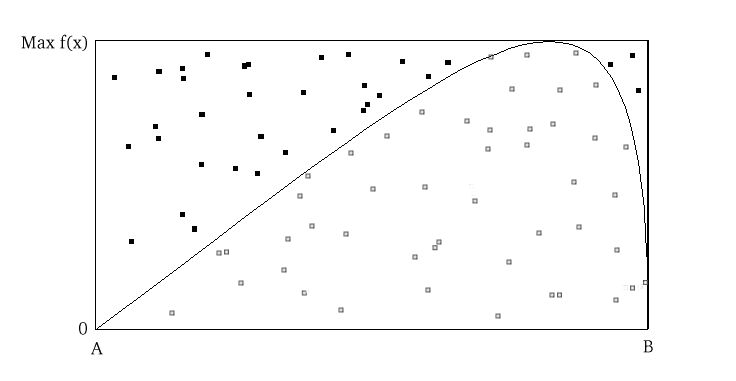
\includegraphics[scale=0.4]{reject.png}
    \end{center}
    \caption{Rejection sampling of a bounded form. Area is estimated by the ratio of accepted (open squares) to total points, multiplied by the rectangle area.}
    \label{fig:bound}
\end{figure}

Posit a function, $f(x)$ which can be evaluated for any value on the support of $x:S_x = [A,B]$, but may not be integrable or easily sampled from. If we can calculate the maximum  value of $f(x)$, we can then define a rectangle that is guaranteed to contain all possible values $(x,f(x))$. It is then trivial to generate points over the box and enumerate the values that fall under the curve (Figure \ref{fig:bound}).

\[
\frac{\mbox{Points under curve}}{\mbox{Points generated}} \times \mbox{box area} = \lim_{n \to \infty} \int_A^B f(x) dx
\]

\begin{figure}[h]
        \begin{center}
        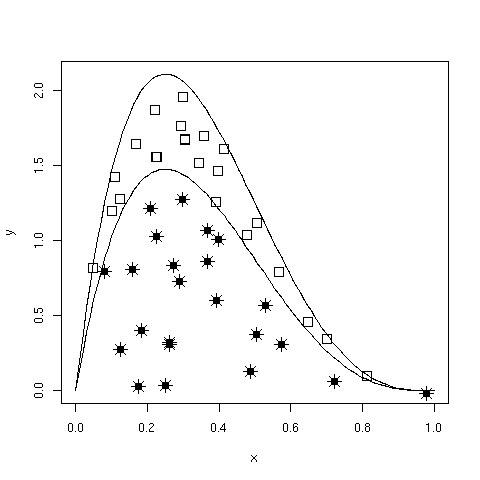
\includegraphics[scale=0.4]{envelope.png}
    \end{center}
    \caption{Rejection sampling of an unbounded form using an enveloping distribution.}
    \label{fig:unbound}
\end{figure}

\noindent This approach is useful, for example, in estimating the normalizing constant for posterior distributions.

If $f(x)$ has unbounded support (i.e. infinite tails), such as a Gaussian distribution, a bounding box is no longer appropriate. We must specify a majorizing (or, enveloping) function, $g(x)$, which implies:

\[
g(x) \ge  f(x) \qquad\forall x \in (-\infty,\infty)
\]

Having done this, we can now sample ${x_i}$ from $g(x)$ and accept or reject each of these values based upon $f(x_i)$. Specifically, for each draw $x_i$, we also draw a uniform random variate $u_i$ and accept $x_i$ if $u_i < f(x_i)/cg(x_i)$, where $c$ is a constant (Figure \ref{fig:unbound}). This approach is made more efficient by choosing an enveloping distribution that is ``close'' to the target distribution, thus maximizing the number of accepted points. Further improvement is gained by using optimized algorithms such as importance sampling which, as the name implies, samples more frequently from important areas of the distribution.

Rejection sampling is usually subject to declining performance as the dimension of the parameter space increases, so it is used less frequently than MCMC for evaluation of posterior distributions \citep{Gamerman:1997tb}.

%___________________________________________________________________________

\hypertarget{markov-chains}{}
\pdfbookmark[0]{Markov Chains}{markov-chains}
\section{Markov Chains}

A Markov chain is a special type of \emph{stochastic process}. The standard definition of a stochastic process is an ordered collection of random variables:

\[
\{X_t:t \in T\}
\]

\noindent where $t$ is frequently (but not necessarily) a time index. If we think of $X_t$ as a state $X$ at time $t$, and invoke the following dependence condition on each state:

\[
Pr(X_{t+1}=x_{t+1} | X_t=x_t, X_{t-1}=x_{t-1},\ldots,X_0=x_0) = Pr(X_{t+1}=x_{t+1} | X_t=x_t)
\]

\noindent then the stochastic process is known as a Markov chain. This conditioning specifies that the future depends on the current state, but not past states. Thus, the Markov chain wanders about the state space, remembering only where it has just been in the last time step. The collection of transition probabilities is sometimes called a \emph{transition matrix} when dealing with discrete states, or more generally, a \emph{transition kernel}. 

\noindent In the context of Markov chain Monte Carlo, it is useful to think of the Markovian property as ``mild non-independence''. MCMC allows us to indirectly generate independent samples from a particular posterior distribution.

%___________________________________________________________________________

\hypertarget{jargon-busting}{}
\pdfbookmark[1]{Jargon-busting}{jargon-busting}
\subsection{Jargon-busting}

Before we move on, it is important to define some general properties of Markov chains. They are frequently encountered in the MCMC literature, and some will help us decide whether MCMC is producing a useful sample from the posterior.

\begin{itemize}
\item \emph{Homogeneity}: A Markov chain is homogeneous at step $t$ if the transition probabilities are independent of time $t$.
\item \emph{Irreducibility}: A Markov chain is irreducible if every state is accessible in one or more steps from any other state. That is, the chain contains no absorbing states. This implies that there is a non-zero probability of eventually reaching state $k$ from any other state in the chain.
\item \emph{Recurrence}: States which are visited repeatedly are \emph{recurrent}. If the expected time to return to a particular state is bounded, this is known as \emph{positive recurrence}, otherwise the recurrent state is \emph{null recurrent}. Further, a chain is \emph{Harris recurrent} when it visits all states $X \in S$ infinitely often in the limit as $t \to \infty$; this is an important characteristic when dealing with unbounded, continuous state spaces. Whenever a chain ends up in a closed, irreducible set of Harris recurrent states, it stays there forever and visits every state with probability one.
\item \emph{Stationarity}: A stationary Markov chain produces the same marginal distribution when multiplied by the transition kernel.  Thus, if $P$ is some $n \times n$ transition matrix:

\[{\bf \pi P} = {\bf \pi}\]

\noindent for Markov chain $\pi$. Thus, $\pi$ is no longer subscripted, and is referred to as the \emph{limiting distribution} of the chain. In MCMC, the chain explores the state space according to its limiting marginal distribution.
\item \emph{Ergodicity}: Ergodicity is an emergent property of Markov chains which are irreducible, positive Harris recurrent and aperiodic. Ergodicity is defined as:

\[
\lim_{n \to \infty} Pr^{(n)}(\theta_i \rightarrow \theta_j) = \pi(\theta) \quad \forall \theta_i, \theta_j \in \Theta
\]

\noindent or in words, after many steps the marginal distribution of the chain is the same at one step as at all other steps. This implies that our Markov chain, which we recall is dependent, can generate samples that are independent if we wait long enough between samples. If it means anything to you, ergodicity is the analogue of the strong law of large numbers for Markov chains. For example, take values $\theta_{i+1},\ldots,\theta_{i+n}$ from a chain that has reached an ergodic state. A statistic of interest can then be estimated by:

\[
\frac{1}{n}\sum_{j=i+1}^{i+n} h(\theta_j) \approx \int f(\theta) h(\theta) d\theta
\]

\end{itemize}

%___________________________________________________________________________

\hypertarget{reversible-markov-chains}{}
\pdfbookmark[0]{Why MCMC Works: Reversible Markov Chains}{reversible-markov-chains}
\section{Why MCMC Works: Reversible Markov Chains}

Markov chain Monte Carlo simulates a Markov chain for which some function of interest (\emph{e.g.} the joint distribution of the parameters of some model) is the unique, invariant limiting distribution. An invariant distribution with respect to some Markov chain with transition kernel $Pr(y \mid x)$ implies that:
\[
\int_x Pr(y \mid x) \pi(x) dx = \pi(y).
\]

Invariance is guaranteed for any \textbf{reversible} Markov chain. Consider a Markov chain in reverse sequence: $\{\theta^{(n)},\theta^{(n-1)},...,\theta^{(0)}\}$. This sequence is still Markovian, because:
\[
Pr(\theta^{(k)}=y \mid \theta^{(k+1)}=x,\theta^{(k+2)}=x_1,\ldots ) = Pr(\theta^{(k)}=y \mid \theta^{(k+1)}=x)
\]
Forward and reverse transition probabilities may be related through Bayes theorem:
\begin{eqnarray}
Pr(\theta^{(k)}=y \mid \theta^{(k+1)}=x) &=& \frac{Pr(\theta^{(k+1)}=x \mid \theta^{(k)}=y) Pr(\theta^{(k)}=y)}{Pr(\theta^{(k+1)}=x)} \nonumber \\
&=& \frac{Pr(\theta^{(k+1)}=x \mid \theta^{(k)}=y) \pi^{(k)}(y)}{\pi^{(k+1)}(x)} \nonumber
\end{eqnarray}

\[
\frac{Pr(\theta^{(k+1)}=x \mid \theta^{(k)}=y) \pi^{(k)}(y)}{\pi^{(k+1)}(x)}
\]

\noindent Though not homogeneous in general, $\pi$ becomes homogeneous if \textbf{Do you ever call the stationary distribution itself homogeneous?}:
\begin{itemize}
\item $n \rightarrow \infty$
\item $\pi^{(0)}=\pi$ for some $i < k$ \textbf{Is it meant to be $\pi^(i)$, and }
\end{itemize}

\noindent If this chain is homogeneous it is called reversible, because it satisfies the \textbf{detailed balance equation}:
\[
\pi(x)Pr(y \mid x) = \pi(y) Pr(x \mid y)
\]
Reversibility is important because it has the effect of balancing movement through the entire state space. When a Markov chain is reversible, $\pi$ is the unique, invariant, stationary distribution of that chain.
Hence, if $\pi$ is of interest, we need only find the reversible Markov chain for which $\pi$ is the limiting distribution. This is what MCMC does!

%___________________________________________________________________________

\hypertarget{gibbs-sampling}{}
\pdfbookmark[0]{Gibbs Sampling}{gibbs-sampling}
\section{Gibbs Sampling}

The Gibbs sampler is the simplest and most prevalent MCMC algorithm. If a posterior has $k$ parameters to be estimated, we may condition each parameter on current values of the other $k-1$ parameters, and sample from the resultant distributional form (usually easier), and repeat this operation on the other parameters in turn. This procedure generates samples from the posterior distribution. Note that we have now combined Markov chains (conditional independence) and Monte Carlo techniques (estimation by simulation) to yield Markov chain Monte Carlo.

Here is a stereotypical Gibbs sampling algorithm:

\newcounter{lcount}
\begin{list}{\arabic{lcount}}
{\usecounter{lcount}}
\item Choose starting values for states (parameters): ${\bf \theta} = [\theta_1^{(0)},\theta_2^{(0)},\ldots,\theta_k^{(0)}]$
\item Initialize counter $j=1$
\item Draw the following values from each of the $k$ conditional distributions:
\begin{eqnarray*}
\theta_1^{(j)} &\sim& \pi(\theta_1 | \theta_2^{(j-1)},\theta_3^{(j-1)},\ldots,\theta_{k-1}^{(j-1)},\theta_k^{(j-1)}) \\
\theta_2^{(j)} &\sim& \pi(\theta_2 | \theta_1^{(j)},\theta_3^{(j-1)},\ldots,\theta_{k-1}^{(j-1)},\theta_k^{(j-1)}) \\
\theta_3^{(j)} &\sim& \pi(\theta_3 | \theta_1^{(j)},\theta_2^{(j)},\ldots,\theta_{k-1}^{(j-1)},\theta_k^{(j-1)}) \\
\vdots \\
\theta_{k-1}^{(j)} &\sim& \pi(\theta_{k-1} | \theta_1^{(j)},\theta_2^{(j)},\ldots,\theta_{k-2}^{(j)},\theta_k^{(j-1)}) \\
\theta_k^{(j)} &\sim& \pi(\theta_k | \theta_1^{(j)},\theta_2^{(j)},\theta_4^{(j)},\ldots,\theta_{k-2}^{(j)},\theta_{k-1}^{(j)})
\end{eqnarray*}
\item Increment $j$ and repeat until convergence occurs.
\end{list}

As we can see from the algorithm, each distribution is conditioned on the last iteration of its chain values, constituting a Markov chain as advertised. The Gibbs sampler has all of the important properties outlined in the previous section: it is aperiodic, homogeneous and ergodic. Once the sampler converges, all subsequent samples are from the target distribution. This convergence occurs at a geometric rate.

\hypertarget{the-metropolis-hastings-algorithm}{}
\pdfbookmark[0]{The Metropolis-Hastings Algorithm}{the-metropolis-hastings-algorithm}
\section{The Metropolis-Hastings Algorithm}

The key to success in applying the Gibbs sampler to the estimation of Bayesian posteriors is being able to specify the form of the complete conditionals of ${\bf \theta}$. In fact, the algorithm cannot be implemented without them. Of course, the posterior conditionals cannot always be neatly specified. In contrast to the Gibbs algorithm, the Metropolis-Hastings algorithm generates candidate state transitions from an alternate distribution, and accepts or rejects each candidate probabilistically.

Let us first consider a simple Metropolis-Hastings algorithm for a single parameter, $\theta$. We will use a standard sampling distribution, referred to as the \emph{proposal distribution}, to produce candidate variables $q_t(\theta^{\prime} | \theta)$. That is, the generated value, $\theta^{\prime}$, is a \emph{possible} next value for $\theta$ at step $t+1$. We also need to be able to calculate the probability of moving back to the original value from the candidate, or $q_t(\theta | \theta^{\prime})$. These probabilistic ingredients are used to define an \emph{acceptance ratio}:

\[
a(\theta^{\prime},\theta) = \frac{q_t(\theta^{\prime} | \theta) \pi(\theta^{\prime})}{q_t(\theta | \theta^{\prime}) \pi(\theta)}
\]

\noindent The value of $\theta^{(t+1)}$ is then determined by:

\[
\theta^{(t+1)} = \left\{\begin{array}{l@{\quad \mbox{with prob.} \quad}l}\theta^{\prime} & \min(a(\theta^{\prime},\theta),1) \\ \theta^{(t)} & 1 - \min(a(\theta^{\prime},\theta),1) \end{array}\right.
\]

\noindent This transition kernel implies that movement is not guaranteed at every step. It only occurs if the suggested transition is likely based on the acceptance ratio.

A single iteration of the Metropolis-Hastings algorithm proceeds as follows:

\newcounter{lcount2}
\begin{list}{\arabic{lcount2}}
{\usecounter{lcount2}}
\item Sample $\theta^{\prime}$ from $q(\theta^{\prime} | \theta^{(t)})$.
\item Generate a Uniform[0,1] random variate $u$.
\item If $a(\theta^{\prime},\theta) > u$ then $\theta^{(t+1)} = \theta^{\prime}$, otherwise $\theta^{(t+1)} = \theta^{(t)}$.
\end{list}

\noindent The original form of the algorithm specified by Metropolis required that $q_t(\theta^{\prime} | \theta) = q_t(\theta | \theta^{\prime})$, which reduces $a(\theta^{\prime},\theta)$ to $\pi(\theta^{\prime})/\pi(\theta)$, but this is not necessary. In either case, the state moves to high-density points in the distribution with high probability, and to low-density points with low probability. After convergence, the Metropolis-Hastings algorithm describes the full target posterior density, so all points are recurrent.

%___________________________________________________________________________

\hypertarget{random-walk-metropolis-hastings}{}
\pdfbookmark[1]{Random-walk Metropolis-Hastings}{random-walk-metropolis-hastings}
\subsection{Random-walk Metropolis-Hastings}

A practical implementation of the Metropolis-Hastings algorithm makes use of a random-walk proposal. Recall that a random walk is a Markov chain that evolves according to:

\begin{eqnarray*}
\theta^{(t+1)} &=& \theta^{(t)} + \epsilon_t \\
\epsilon_t &\sim& f(\phi)
\end{eqnarray*}

As applied to the MCMC sampling, the random walk is used as a proposal distribution, whereby dependent proposals are generated according to:

\[
q(\theta^{\prime} | \theta^{(t)}) = f(\theta^{\prime} - \theta^{(t)}) = \theta^{(t)} + \epsilon_t
\]

Generally, the density generating $\epsilon_t$ is symmetric about zero, resulting in a symmetric chain. Chain symmetry implies that $q(\theta^{\prime} | \theta^{(t)}) = q(\theta^{(t)} | \theta^{\prime})$, which reduces the Metropolis-Hastings acceptance ratio to:

\[
a(\theta^{\prime},\theta) = \frac{\pi(\theta^{\prime})}{\pi(\theta)}
\]

The choice of the random walk distribution for $\epsilon_t$ is frequently a normal or Student's $t$ density, but it may be any distribution that generates an irreducible proposal chain.

An important consideration is the specification of the scale parameter for the random walk error distribution. Large values produce random walk steps that are highly exploratory, but tend to produce proposal values in the tails of the target distribution, potentially resulting in very small acceptance rates. Conversely, small values tend to be accepted more frequently, since they tend to produce proposals close to the current parameter value, but may result in chains that mix very slowly. Some simulation studies suggest optimal acceptance rates in the range of 20-50\%. It is often worthwhile to optimize the proposal variance by iteratively adjusting its value, according to observed acceptance rates early in the MCMC simulation \citep{Gamerman:1997tb}.


\chapter{Building models}
\label{chap:modelbuilding} 
%!TEX root = guide2.0.tex

% \section{Summary}\label{sec:PyMCObjects}
Bayesian inference begins with specification of a probability model relating unknown variables to data. PyMC provides three basic building blocks for Bayesian probability models: \texttt{Stochastic}, \texttt{Deterministic} and \texttt{Potential}. 

A \texttt{Stochastic} object represents a variable whose value is not completely determined by its parents, and a \texttt{Deterministic} object represents a variable that is entirely determined by its parents. In object-oriented programming parlance, \texttt{Stochastic} and \texttt{Deterministic} are subclasses of the \texttt{Variable} class, which is essentially a template for more specific subclasses that are actually implemented in models. The third basic class, representing `factor potentials' (\cite{dawidmarkov,Jordan:2004p5439}), represents an arbitrary log-probability term. \texttt{Potential} and \texttt{Variable}, in turn, are subclasses of \texttt{Node}.

% TODO: Need a better description of what a Potential is. Given the description of Stochastic and Deterministic we have given, its not clear where Potential fits in, as it classifies the world into 2 things -- completely determined by parents and not.

% PyMC also provides container classes for variables to make it easier to program of certain dependency situations, such as when a variable is defined by its dependence on an entire Markov chain.

\medskip
PyMC probability models are simply linked groups of \texttt{Stochastic}, \texttt{Deterministic} and \texttt{Potential} objects. These objects have very limited awareness of the models in which they are embedded and do not themselves possess methods for updating their values in fitting algorithms. Objects responsible for fitting probability models are described in chapter \ref{chap:modelfitting}.
 

\hypertarget{stochastic}{}
\section*{The \texttt{Stochastic} class} \label{stochastic}
\pdfbookmark[0]{The Stochastic class}{stochastic}

A stochastic variable has the following major attributes: 
\begin{description}
    \item[\texttt{value}:] The variable's current value.
    \item[\texttt{logp}:] The log-probability of the variable's current value given the values of its parents.
\end{description}
A stochastic variable can optionally be endowed with a method called \texttt{\bfseries random}, which draws a value for the variable given the values of its parents\footnote{Note that the \texttt{random} method does not provide a Gibbs sample unless the variable has no children.}. Stochastic objects have the following additional attributes that are generally specified automatically, or only specified under particular circumstances:
\begin{description}
    \item[\texttt{parents}:] A dictionary containing the variable's parents. The keys of the dictionary correspond to the names assigned to the variable's parents by the variable, and the values correspond to the actual parents. For example, the keys of $s$'s parents dictionary in model (\ref{disastermodel}) would be \texttt{'t_l'} and \texttt{'t_h'}. Thanks to Python's dynamic typing, the actual parents (\emph{i.e.} the values of the dictionary) may be of any class or type.
    \item[\texttt{children}:] A set containing the variable's children. This set is produced automatically; the user doesn't need to worry about filling it.
    \item[\texttt{extended_parents}:] A set containing all the stochastic variables on which the variable depends either directly or via a sequence of deterministic variables. If the value of any of these variables changes, the variable will need to recompute its log-probability. This set is produced automatically.
    \item[\texttt{extended_children}:] A set containing all the stochastic variables and potentials that depend on the variable either directly or via a sequence of deterministic variables. If the variable's value changes, all of these variables will need to recompute their log-probabilities. This set is produced automatically.
    \item[\texttt{coparents}:] A set containing all the stochastic variables that share extended children with the variable.
    \item[\texttt{moral_neighbors}:] A set containing the union of the variable's extended parents, extended children and coparents, with Potential objects removed.
    \item[\texttt{markov_blanket}:] A set containing self and self's moral neighbors.
    \item[\texttt{isdata}:] A flag (boolean) indicating whether the variable's value has been observed (is fixed).
    \item[\texttt{dtype}:] A Numpy dtype object (such as \texttt{numpy.int}) that specifies the type of the variable's value to fitting methods. If this is \texttt{None} (default) then no type is enforced.
    % \item[\texttt{__name__}:] The name of the variable, should be unique.
    %    \item[\texttt{__doc__}:] The docstring of the variable.
\end{description}

\subsection{Creation of stochastic variables}
There are three main ways to create stochastic variables, called the \textbf{automatic}, \textbf{decorator}, and \textbf{direct} interfaces.

\begin{description}    
    \item[Automatic] Stochastic variables with standard distributions provided by PyMC (see chapter \ref{chap:distributions} ) can be created in a single line using special subclasses of \texttt{Stochastic}. For example, the uniformly-distributed discrete variable $s$ in (\ref{disastermodel}) could be created using the automatic interface as follows:
    \begin{verbatim}
        s = DiscreteUniform('s', 1851, 1962, value=1900)
    \end{verbatim}

    In addition to the classes in chapter \ref{chap:distributions}, \texttt{scipy.stats.distributions}' random variable classes are wrapped as \texttt{Stochastic} subclasses if SciPy is installed. These distributions are in the submodule \texttt{pymc.SciPyDistributions}

    Users can call the class factory \texttt{stochastic_from_dist} to produce \texttt{Stochastic} subclasses of their own from probability distributions not included with PyMC.%  These classes' init methods take the following arguments:
    % \begin{description}
    %     \item[\texttt{name}:] The name of the variable.
    %     \item[\texttt{value}:] An initial value for the variable.
    %     \item[\texttt{parents}:] Keyword arguments specifying the parents of the variable.
    %     \item[\texttt{isdata} (optional)]
    %     \item[\texttt{doc} (optional):] The docstring of the variable.
    %     \item[\texttt{verbose} (optional):] An integer from 0 to 3.
    %     \item[\texttt{trace} (optional):] A boolean indicating whether a trace should be kept for this variable in Monte Carlo fitting methods.
    %     \item[\texttt{cache_depth}:] See section \ref{sec:caching}. 
    % \end{description}
    
    
    \item[Decorator] Uniformly-distributed discrete stochastic variable $s$ in (\ref{disastermodel}) could be created as follows:
    \begin{verbatim}
@stochastic(dtype=int)
def s(value=1900, t_l=1851, t_h=1962):
    """The switchpoint for the rate of disaster occurrence."""
    if value > t_h or value < t_l:
        return -Inf
    else:
        return -log(t_h - t_l + 1) 
    \end{verbatim}
Note that this is a simple Python function, preceded by a Python expression called a \textbf{decorator}, here called \texttt{@stochastic}. Generally, decorators enhance functions with additional properties or functionality. The \texttt{Stochastic} object produced by the \texttt{@stochastic} decorator will evaluate its log-probability using the function \texttt{s}. The \texttt{value} argument, which is required, provides an initial value for the variable. The remaining arguments will be assigned as parents of \texttt{s} (\emph{i.e.} they will populate the \texttt{parents} dictionary).

The \texttt{value} and parents of stochastic variables may be any objects, provided their log-probability functions return a real number (Numpy \texttt{float}). PyMC and SciPy both provide fast implementations of several standard probability distributions that may be helpful for creating custom stochastic variables.

    The decorator \texttt{stochastic} can take several arguments: 
    \begin{itemize}
        \item A flag called \texttt{trace}, which signals to \texttt{MCMC} instances whether an MCMC trace should be kept for the stochastic variable. \texttt{@stochastic(trace = False)} would turn tracing off. Defaults to \texttt{True}.
        \item A flag called \texttt{plot}, which signals to \texttt{MCMC} instances whether summary plots should be produced for this variable. Defaults to \texttt{True}.
        \item An integer-valued argument called \texttt{verbose} that controls the amount of output the variable prints to the screen. The default is $0$, no output; the maximum value is $3$. 
        \item A Numpy datatype called \texttt{dtype}. Decorating a log-probability function with \texttt{@stochastic(dtype=int)} would produce a discrete random variable. Such a variable will cast its value to either an integer or an array of integers. The default dtype is \texttt{float}.
    \end{itemize} 

    The decorator interface has a slightly more complex implementation which allows you to specify a \texttt{random} method for sampling the stochastic variable's value conditional on its parents.
    \begin{verbatim}
@stochastic(dtype=int)
def s(value=1900, t_l=1851, t_h=1962):
    """The switchpoint for the rate of disaster occurrence."""

    def logp(value, t_l, t_h):
        if value > t_h or value < t_l:
            return -Inf
        else:
            return -log(t_h - t_l + 1) 
            
    def random(t_l, t_h):
        return round( (t_l - t_h) * random() ) + t_l

    rseed = 1.
    \end{verbatim}
The stochastic variable again gets its name, docstring and parents from function $s$, but in this case it will evaluate its log-probability using the \texttt{logp} function. The \texttt{random} function will be used when \texttt{s.random()} is called. Note that \texttt{random} doesn't take a \texttt{value} argument, as it generates values itself. The optional \texttt{rseed} variable provides a seed for the random number generator. The stochastic's \texttt{value} argument is optional when a \texttt{random} method is provided; if no initial value is provided, it will be drawn automatically using the \texttt{random} method.

    \item[Direct] It's possible to instantiate \texttt{Stochastic} directly:
\begin{verbatim}
def s_logp(value, t_l, t_h):
    if value > t_h or value < t_l:
        return -Inf
    else:
        return -log(t_h - t_l + 1) 

def s_rand(t_l, t_h):
    return round( (t_l - t_h) * random() ) + t_l

s = Stochastic( logp = s_logp, 
                doc = 'The switchpoint for the rate of disaster occurrence.',
                name = 's', 
                parents = {'t_l': 1851, 't_h': 1962},
                random = s_rand,                 
                trace = True,                 
                value = 1900,
                dtype=int,
                rseed = 1., 
                isdata = False,
                cache_depth = 2,
                plot=True,
                verbose = 0)
\end{verbatim}
Notice that the log-probability and random variate functions are specified externally and passed to \texttt{Stochastic} as arguments. This is a rather awkward way to instantiate a stochastic variable; consequently, such implementations should be rare.

\end{description}


\hypertarget{sub:warning}{}
\subsection*{Don't update stochastic variables' values in-place} \label{sub:warning}
\pdfbookmark[0]{Don't update stochastic variables' values in-place}{sub:warning}

\texttt{Stochastic} objects' values should not be updated in-place. This confuses PyMC's caching scheme and corrupt the process used for accepting or rejecting proposed values in the MCMC algorithm. The only way a stochastic variable's value should be updated is using statements of the following form:
\begin{verbatim}
    A.value = new_value
\end{verbatim}
The following are in-place updates and should \emph{never} be used:
\begin{itemize}
    \item \texttt{A.value += 3}
    \item \texttt{A.value[2,1] = 5}
    \item \texttt{A.value.attribute = new_attribute_value}.
\end{itemize}

This restriction becomes onerous if a step method proposes values for the elements of an array-valued variable separately. In this case, it may be preferable to partition the variable into several variables stored in an array or list.


\hypertarget{data}{}
\section*{Data} \label{data}
\pdfbookmark[0]{Data}{data}

Although the data $D$ is represented by a random variable in the model, we have fixed its value by observing it. Such variables are represented by \texttt{Stochastic} objects whose \texttt{isdata} attribute is set to \texttt{True}. If a stochastic variable's \texttt{isdata} flag is \texttt{True}, its value cannot be changed.

\subsection*{Declaring stochastic variables to be data}

In the short and long interfaces, a \texttt{Stochastic} object's \texttt{isdata} flag can be set to true by stacking a \texttt{@data} decorator on top of the \texttt{@stochastic} decorator:
\begin{verbatim}
@data
@stochastic(dtype=int)
def D(value = count_array, switchpoint = s, early_rate = e, late_rate = l):
    """The observed annual disaster counts."""
    logp = sum(-value[:switchpoint]) + early_rate * log(value[:switchpoint]) \
            - gammaln(early_rate))
    logp += sum(-value[switchpoint:] + late_rate * log(value[switchpoint:]) \
            - gammaln(late_rate))
    return logp
\end{verbatim}
In the automatic and direct interfaces, the \texttt{isdata} argument can be simply set to \texttt{True}.


\hypertarget{deterministic}{}
\section*{The \texttt{Deterministic} class} \label{deterministic}
\pdfbookmark[0]{The Deterministic class}{deterministic}

The \texttt{Deterministic} class represents variables whose values are completely determined by the values of their parents. For example, in model (\ref{disastermodel}), $r$ is a deterministic variable. Recall it was defined by
\begin{eqnarray*}
    r_t=\left\{\begin{array}{ll}
        e & t\le s\\ l & t>s
        \end{array}\right.,
\end{eqnarray*}
so $r$'s value can be computed exactly from the values of its parents $e$, $l$ and $s$.

A deterministic variable's most important attribute is \texttt{\bfseries value}, which gives the current value of the variable given the values of its parents. Like \texttt{Stochastic}'s \texttt{logp} attribute, this attribute is computed on-demand and cached for efficiency.

A Deterministic variable has the following additional attributes:
\begin{description}
    \item[\texttt{parents}:] A dictionary containing the variable's parents. The keys of the dictionary correspond to the names assigned to the variable's parents by the variable, and the values correspond to the actual parents. Thanks to Python's dynamic typing, parents may be of any class or type.
    \item[\texttt{children}:] A set containing the variable's children, which must be nodes. This set is produced automatically; the user doesn't need to worry about filling it.
    % \item[\texttt{__name__}:] The name of the variable, should be unique.
    %     \item[\texttt{__doc__}:] The docstring of the variable.
\end{description}
Deterministic variables have no methods.


\subsection*{Creation of deterministic variables}
Deterministic variables are less complicated than stochastic variables, and have similar \textbf{automatic}, \textbf{decorator}, and \textbf{direct} interfaces:
\begin{description}
   \item[Automatic] A handful of common functions have been wrapped in Deterministic objects. These are brief enough to list:
   \begin{description}
      \item[\texttt{LinearCombination}:] Has two parents $x$ and $y$, both of which must be iterable (\emph{i.e.} vector-valued). This function returns:
      \[
      \sum_i x_i^{\prime} y_i.
      \]
      \item[\texttt{Index}:] Has three parents $x$, $y$ and \texttt{index}. $x$ and $y$ must be iterables, \texttt{index} must be valued as an integer. Index returns the dot product of $x$ and $y$ for the elements specified by \mathttt{index}:
      \[
      x[\mathtt{index}]^T y[\mathtt{index}].
      \]
      \texttt{Index} is useful for implementing dynamic models, in which the parent-child connections change.
      \item[\texttt{Lambda}:] Converts an anonymous function (in Python, called \textbf{lambda functions}) to a \texttt{Deterministic} instance on a single line.
      \item[\texttt{CompletedDirichlet}:] PyMC represents Dirichlet variables of length $k$ by the first $k-1$ elements; since they must sum to 1, the $k^{th}$ element is determined by the others. \texttt{CompletedDirichlet} appends the $k^{th}$ element to the value of its parent $D$.      
      \item[\texttt{Logit}, \texttt{InvLogit}, \texttt{StukelLogit}, \texttt{StukelInvLogit}:] Various common link functions for generalized linear models.
   \end{description}
   It's a good idea to use these classes when feasible, because certain fitting methods (Gibbs step methods in particular) implicitly know how to take them into account.

    \item[Decorator] A deterministic variable can be created via a decorator in a way very similar to \texttt{Stochastic}'s decorator interface:
\begin{verbatim}
@deterministic
def r(switchpoint = s, early_rate = e, late_rate = l):
    """The rate of disaster occurrence."""
    value = zeros(N)
    value[:switchpoint] = early_rate
    value[switchpoint:] = late_rate
    return value
\end{verbatim}
Notice that rather than returning the log-probability, as is the case for \texttt{Stochastic} objects, the function returns the value of the deterministic object, given its parents. This return value may be of any type, as is suitable for the problem at hand. Arguments' keys and values are converted into a parent dictionary as with \texttt{Stochastic}'s short interface. The \texttt{deterministic} decorator can take \texttt{trace} and \texttt{verbose} arguments, like the \texttt{stochastic} decorator.

Of course, since deterministic nodes are not expected to generate random variates, the longer implementation of the decorator interface available to \texttt{Stochastic} objects is not relevant here.

    \item[Direct] Deterministic objects can also be instantiated directly, by passing the evaluation function to the Deterministic class as an argument:
\begin{verbatim}
def r_eval(switchpoint = s, early_rate = e, late_rate = l):
    value = zeros(N)
    value[:switchpoint] = early_rate
    value[switchpoint:] = late_rate
    return value

r = Deterministic(  eval = r_eval, 
                    name = 'r',
                    parents = {'switchpoint': s, 'early_rate': e, 'late_rate': l}),
                    doc = 'The rate of disaster occurrence.',
                    trace = True,
                    verbose = 0,
                    cache_depth = 2)
\end{verbatim}
The \texttt{trace} flag signals to \texttt{Model} whether to keep a trace for the variable, as with stochastic variables.
\end{description}

Note that deterministic variables have no \texttt{isdata} flag. If a deterministic variable's value were known, its parents would be restricted to the inverse image of that value under the deterministic variable's evaluation function. This usage would be extremely difficult to support in general, but it can be implemented for particular applications at the \texttt{StepMethod} level.

\hypertarget{container}{}
\section*{Containers} \label{container}
\pdfbookmark[0]{Containers}{container}

In some situations, such as a state-space model, it would be inconvenient to assign a unique label to each parent of $y$:
\begin{eqnarray*}
    x_0 &\sim& \textup N(0,\tau_x)\\
    x_{i+1}|x_i &\sim& \textup{N}(x_i, \tau_x)\\
    y|x &\sim& \textup N\left(\sum_{i=0}^{N-1}x_i^2,\tau_y\right)\\
	&&i=0,\ldots, N-2
\end{eqnarray*}
Here, $y$ depends on every element of the Markov chain $x$, but we wouldn't want to manually enter $N$ parent labels \texttt{`x_0'}, \texttt{`x_1'}, etc.

This situation can be handled naturally in PyMC:
\begin{verbatim}
x_0 = Normal(`x_0', mu=0, tau=1)

x = [x_0]
last_x = x_0

for i in range(1,N):          
   x_now = Normal(`x_%i' % i, mu=last_x, tau=1)        
   last_x = x_now 
   x.append(x_now)

@data
@stochastic
def y(value = 1, mu = x, tau = 100):
    mu_sum = 0
    for i in range(N):
        mu_sum += mu[i] ** 2
    return normal_like(value, mu_sum, tau)
\end{verbatim}
PyMC automatically wraps list \texttt{x} in an appropriate \texttt{Container} class. The python expression \texttt{`x_\%i' \% i} labels each Normal object in the container with the appropriate index $i$.

Containers, like variables, have an attribute called \texttt{value}. This attribute returns a copy of the (possibly nested) iterable that was passed into the container function, but with each variable inside replaced with its corresponding value. 

Containers can currently be constructed from lists, tuples, dictionaries, Numpy arrays, modules, sets or any object with a \texttt{__dict__} attribute. Variables and non-variables can be freely mixed in these containers, and different types of containers can be nested\footnote{Nodes whose parents are containers make private shallow copies of those containers. This is done for technical reasons rather than to protect users from accidental misuse.}. Containers attempt to behave like the objects they wrap. All containers are subclasses of \texttt{ContainerBase}. 

Containers have the following useful attributes in addition to \texttt{value}:
\begin{itemize}
    \item\texttt{variables}
    \item\texttt{stochastics}
    \item\texttt{potentials}
    \item\texttt{deterministics}
    \item\texttt{data_stochastics}
    \item\texttt{step_methods}.
\end{itemize}
Each of these attributes is a set containing all the objects of each type in a container, and within any containers in the container.


\hypertarget{potential}{}
\section*{The Potential class} \label{potential}
\pdfbookmark[0]{The Potential class}{potential}

% WE PROBABLY NEED TO GIVE A GOOD EXAMPLE OF WHERE A POTENTIAL IS DIFFERENT FROM A DETERMINISTIC;
% THIS PROBABLY WONT BE CLEAR TO EVERYONE. THE KEY DIFFERENCE IS THAT A POTENTIAL IS PART OF THE
% JOINT POSTERIOR, NO?
% 

The joint density corresponding to model (\ref{disastermodel}) can be written as follows:
\begin{eqnarray*}
    p(D,s,l,e) = p(D|s,l,e) p(s) p(l) p(e).
\end{eqnarray*}
Each factor in the joint distribution is a proper, normalized probability distribution for one of the variables conditional on its parents. Such factors are contributed by \texttt{Stochastic} objects.

In some cases, it's nice to be able to modify the joint density by incorporating terms that don't correspond to probabilities of variables conditional on parents, for example:
\begin{eqnarray*}
    p(x_0, x_2, \ldots x_{N-1}) \propto \prod_{i=0}^{N-2} \psi_i(x_i, x_{i+1}).
\end{eqnarray*}
Arbitrary factors such as $\psi$ are contributed by objects of class \texttt{Potential} (\cite{dawidmarkov} and \cite{Jordan:2004p5439} call these terms `factor potentials'). Bayesian hierarchical notation (cf model (\ref{disastermodel})) doesn't accomodate these potentials. They are most useful in cases where there is no natural dependence hierarchy, such as Markov random fields. They are also useful for expressing `soft data' \citep{Christakos:2002p5506}.

Even when there is a definite dependence hierarchy, potentials can provide a useful shorthand. Consider a new example: we have a dataset $t$ consisting of the days on which several marked animals were recaptured. We believe that the probability $S$ that an animal is not recaptured on any given day can be explained by a covariate vector $x$. We model this situation as follows:
\begin{eqnarray*}
    t_i|S_i \sim \textup{Geometric}(S_i), & i=1\ldots N\\
    S_i = \textup{logit}^{-1}(\beta x_i), &i=1\ldots N\\
    \beta\sim \textup{N}(\mu_\beta, V_\beta).
\end{eqnarray*}
So far, so good. Now suppose we have some knowledge of other related experiments and we have a good idea of what $S$ will be before seeing the data. It's not obvious how to work this prior information in, because as we've written the model $S$ is completely determined by $\beta$. There are three options within the strict Bayesian hierarchical framework:
\begin{itemize}
    \item Work the prior information into the prior on $\beta$.
    \item Incorporate the data from the previous experiments explicitly into the model.
    \item Refactor the model so that $S$ is at the bottom of the hierarchy, and assign the prior directly.
\end{itemize}

Factor potentials provide a convenient way to incorporate the prior information without the need for such major modifications. We can simply modify the joint distribution from
\begin{eqnarray*}
    p(t|S(x,\beta)) p(\beta)
\end{eqnarray*}
to
\begin{eqnarray*}
    \gamma(S,a,b) p(t|S(x,\beta)) p(\beta),
\end{eqnarray*}
where $\gamma$ expresses the prior information. It's a good idea to check the induced priors on $S$ and $\beta$ for sanity. This can be done in PyMC by fitting the model with the data $t$ removed.

\bigskip
Potentials have one important attribute, \texttt{\bfseries logp}, the log of their current probability or probability density value given the values of their parents. The only other additional attribute of interest is \texttt{parents}, a dictionary containing the potential's parents. Potentials have no methods. They have no \texttt{trace} attribute, because they are not variables. They cannot serve as parents of variables (for the same reason), so they have no \texttt{children} attribute.


\subsection*{Creation of \texttt{Potentials}}
There are two ways to create potentials:
\begin{description}
    \item[Decorator] A potential can be created via a decorator in a way very similar to \texttt{Deterministic}'s decorator interface:
\begin{verbatim}
@potential
def psi_i(x_lo = x[i], x_hi = x[i+1]):
    """A pair potential"""
    return -(xlo - xhi)**2
\end{verbatim}
The function supplied should return a Numpy \texttt{float}. The \texttt{potential} decorator can take \texttt{verbose} and \texttt{cache_depth} arguments like the \texttt{stochastic} decorator.
    \item[Direct] The same potential could be created directly as follows:
\begin{verbatim}
def psi_i_logp(x_lo = x[i], x_hi = x[i+1]):
    return -(xlo - xhi)**2
        
psi_i = Potential(  logp = psi_i_logp, 
                    name = 'psi_i',
                    parents = {'xlo': x[i], 'xhi': x[i+1]},
                    doc = 'A pair potential',
                    verbose = 0,
                    cache_depth = 2)
\end{verbatim}
\end{description}


\hypertarget{graphical}{}
\section*{Graphing models} \label{graphical}
\pdfbookmark[0]{Graphing models}{graphical}

The function \texttt{graph} draws graphical representations of \texttt{Model} (Chapter \ref{chap:modelfitting}) instances using GraphViz via the Python package PyDot (if they are installed). See \cite{dawidmarkov} and \cite{Jordan:2004p5439} for more discussion of useful information that can be read off of graphical models. Note that these authors do not consider deterministic variables.

The symbol for stochastic variables is an ellipse. Parent-child relationships are indicated by arrows. These arrows point from parent to child and are labeled with the names assigned to the parents by the children. A graphical representation of model \ref{disastermodel} follows:
\begin{center}
    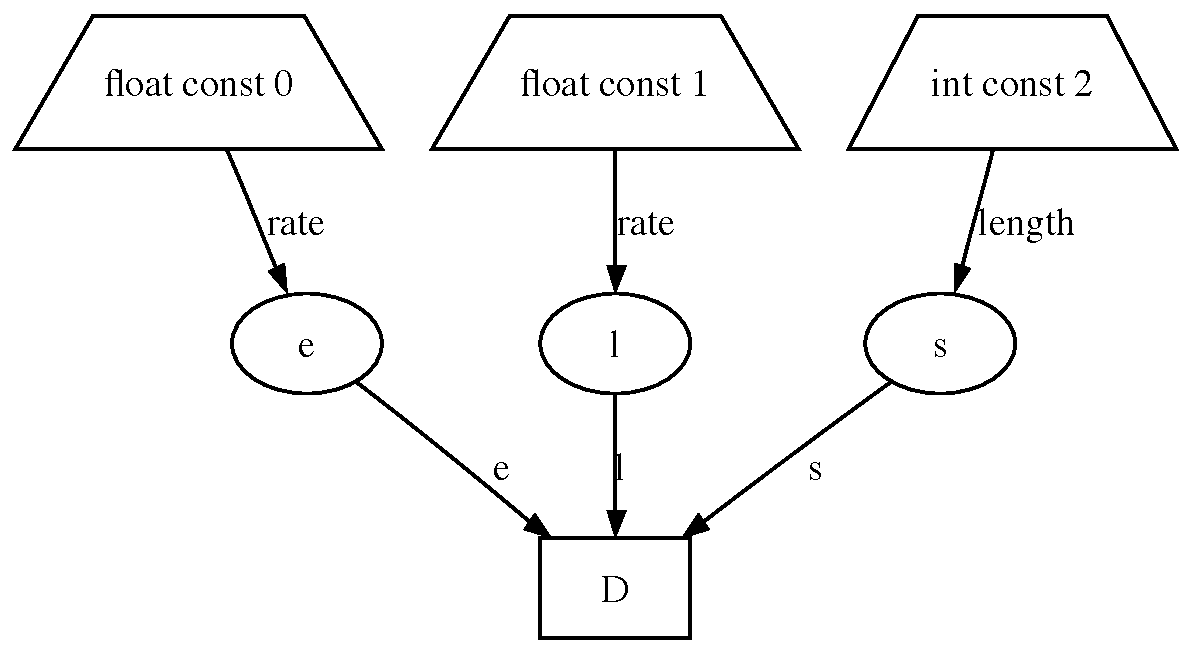
\epsfig{file=DisasterModel.pdf, width=6cm} 
\end{center} 
$D$ is shaded because it is flagged as data.

PyMC's symbol for deterministic variables is a downward-pointing triangle. A graphical representation of model \ref{disastermodel} with $r$ explicit follows:
\begin{center}
    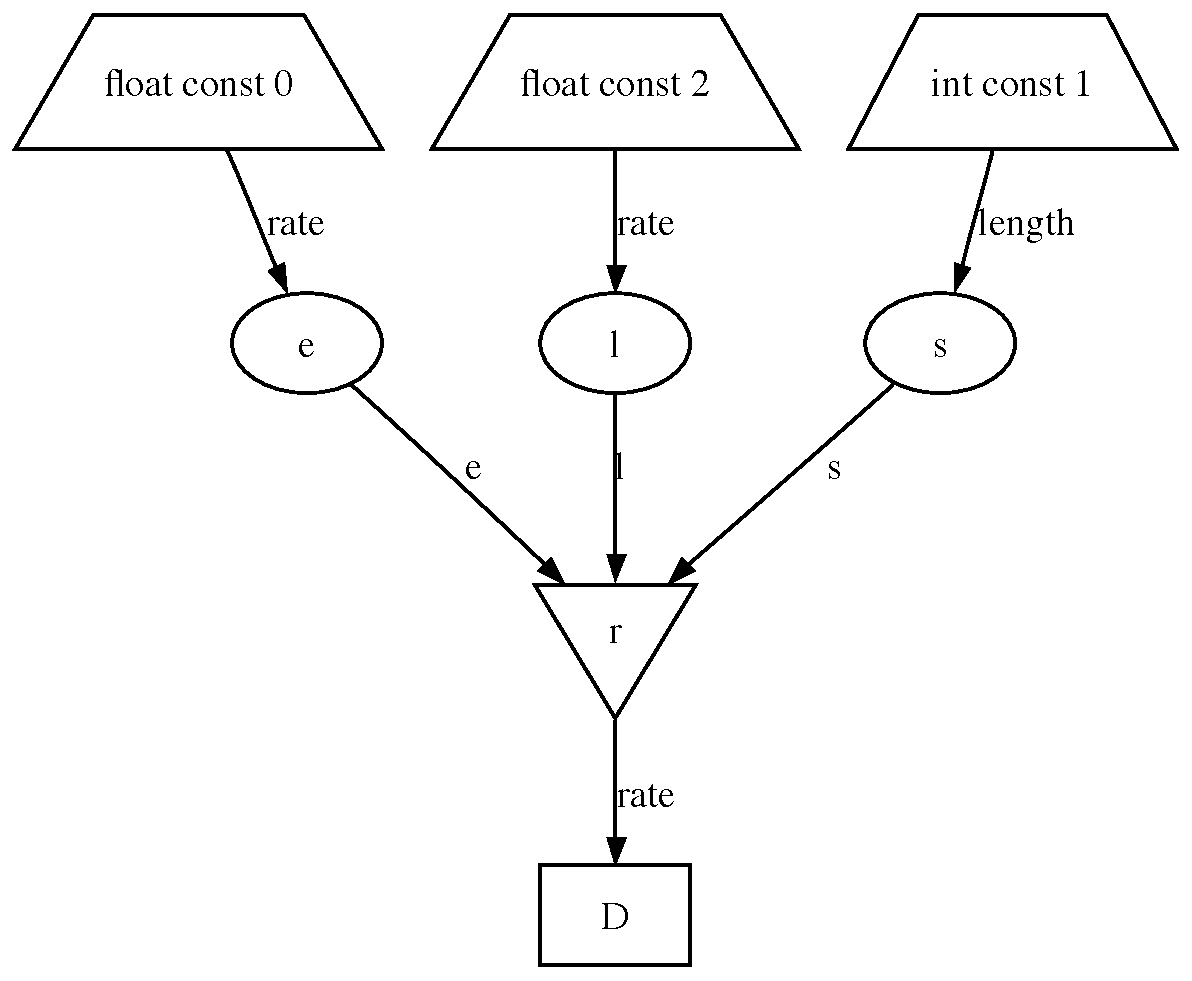
\epsfig{file=DisasterModel2.pdf, width=6cm} 
\end{center}
% Note that if a deterministic variable has more than one child, its parents each inherit all of its children when it is made implicit:
% \begin{center}
%     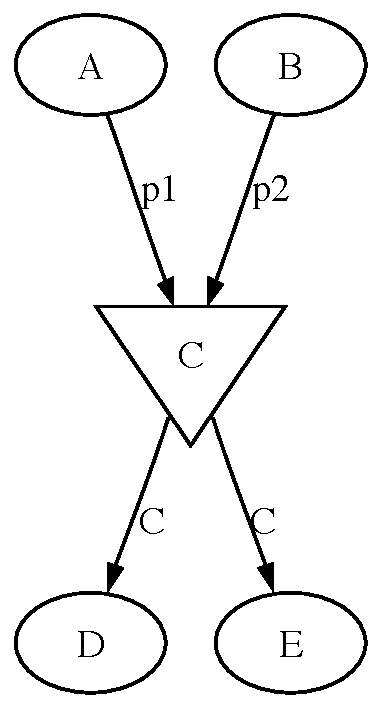
\epsfig{file=DeterministicPreInheritance.pdf, width=3.5cm} $\Rightarrow$ 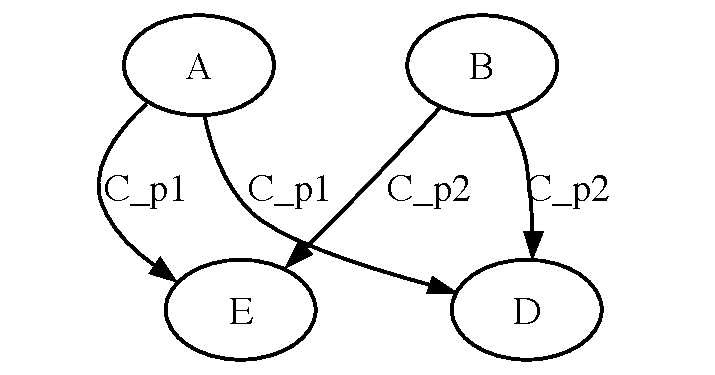
\epsfig{file=DeterministicPostInheritance.pdf, width=5cm}
% \end{center}
% These inherited children can be accessed via the \texttt{extended_children} attributes of the parents.

The symbol for factor potentials is a rectangle:
\begin{center}
    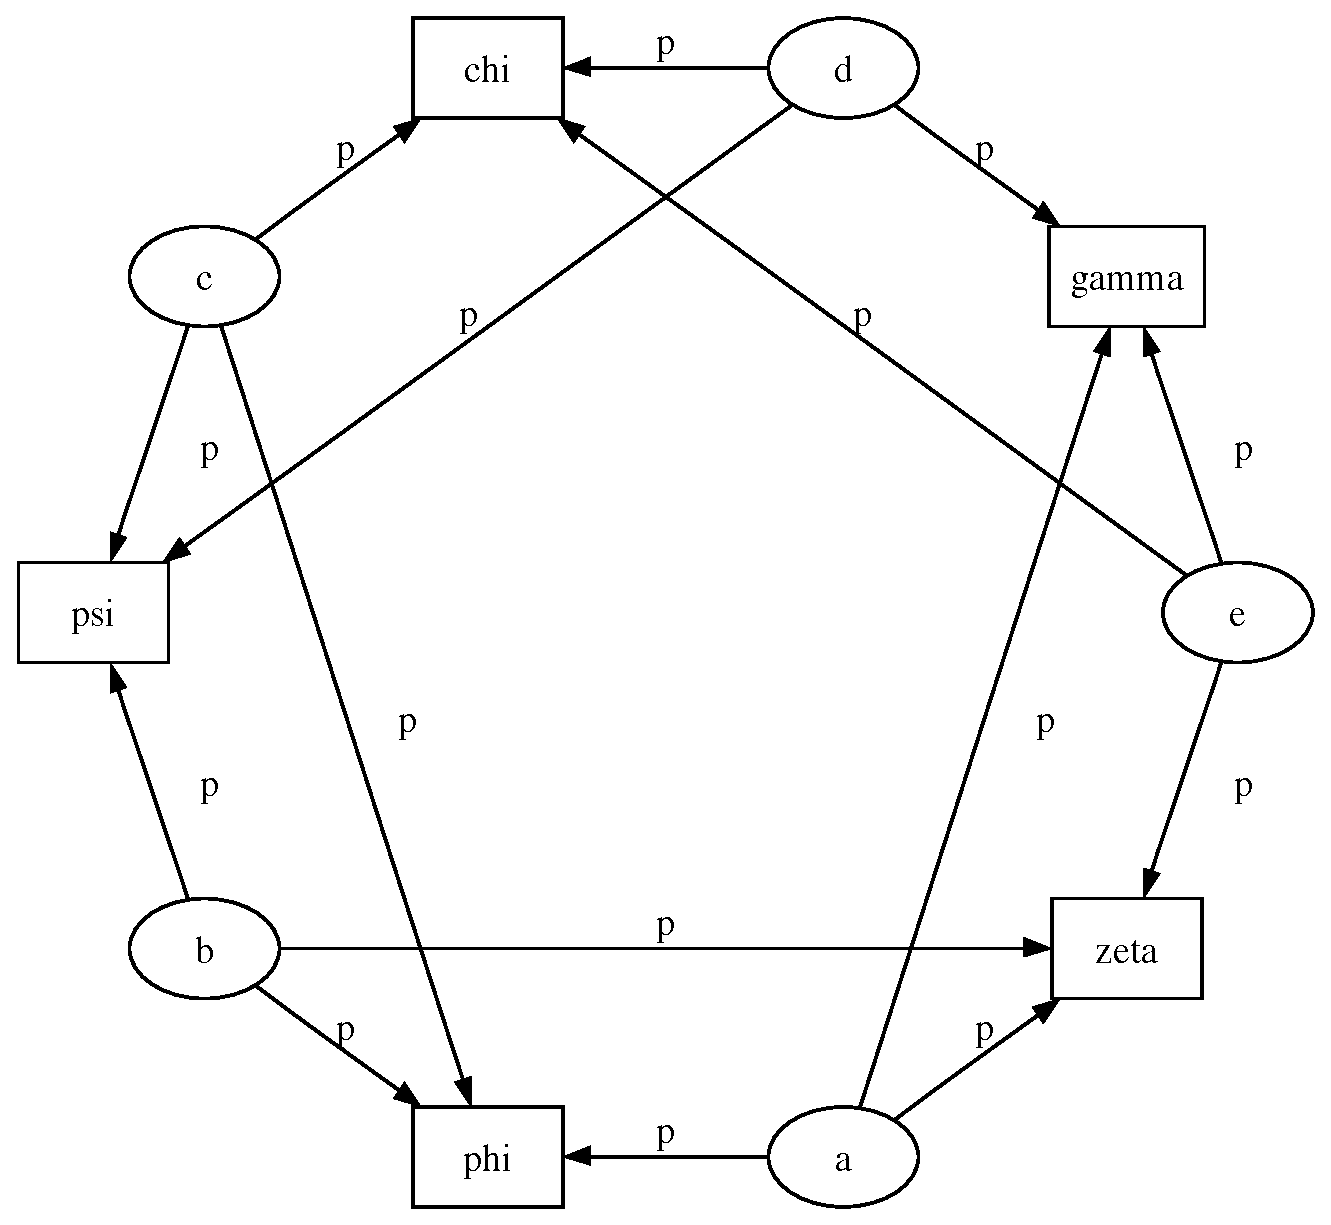
\epsfig{file=PotExample.pdf, width=10cm} 
\end{center}
Factor potentials are usually associated with \emph{undirected} grahical models. In undirected representations, each parent of a potential is connected to every other parent by an undirected edge:
\begin{center}
    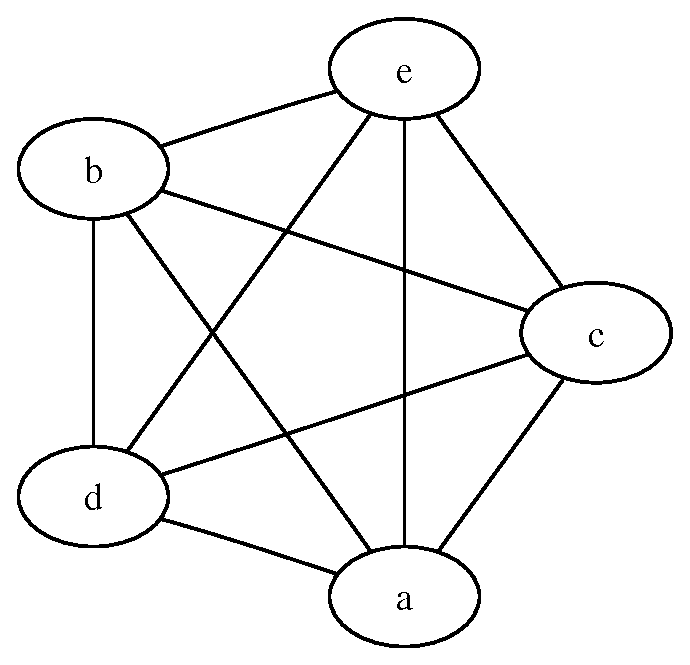
\epsfig{file=PotExampleCollapsed.pdf, width=5cm}
\end{center}

Directed or mixed graphical models can be represented in an undirected form by `moralizing', which is done by the function \texttt{moral_graph}.


\section*{Class \texttt{LazyFunction} and caching}
\label{sec:caching} 

The \texttt{logp} attributes of stochastic variables and potentials and the \texttt{value} attributes of deterministic variables are wrappers for instances of class \texttt{LazyFunction}. Lazy functions are wrappers for ordinary Python functions. A lazy function \texttt{L} could be created from a function \texttt{fun} as follows:
\begin{verbatim}
L = LazyFunction(fun, arguments)
\end{verbatim}
The argument \texttt{arguments} is a dictionary container; \texttt{fun} must accept keyword arguments only. When \texttt{L}'s \texttt{get()} method is called, the return value is the same as the call 
\begin{verbatim}
fun(**arguments.value)
\end{verbatim}
Note that no arguments need to be passed to \texttt{L.get}; lazy functions memorize their arguments.

Before calling \texttt{fun}, \texttt{L} will check the values of \texttt{arguments.variables} against an internal cache. This comparison is done \emph{by reference}, not by value, and this is part of the reason why stochastic variables' values cannot be updated in-place. If \texttt{arguments.variables}' values match a frame of the cache, the corresponding output value is returned and \texttt{fun} is not called. If a call to \texttt{fun} is needed, \texttt{arguments.variables}' values and the return value replace the oldest frame in the cache. The depth of the cache can be set using the optional init argument \texttt{cache_depth}, which defaults to 2.

Caching is helpful in MCMC, because variables' log-probabilities and values tend to be queried multiple times for the same parental value configuration. The default cache depth of 2 turns out to be most useful in Metropolis-Hastings-type algorithms involving proposed values that may be rejected.

Lazy functions are implemented in C using Pyrex, a language for writing Python extensions.

\chapter{Fitting models}
\label{chap:modelfitting}
PyMC probability models are linked collections of nodes. These nodes are only informed by the values of their parents. \code{Deterministic} instances can compute their values given their parents' values, \code{Stochastic} instances can compute their log-probabilities or draw new values, and \code{Potential} instances can compute their log-probabilities. Fitting probability models requires larger-scale coordination and communication.

PyMC provides three objects that fit models:
\begin{itemize}
    \item \code{MCMC}, which coordinates Markov chain Monte Carlo algorithms. The actual work of updating stochastic variables conditional on the rest of the model is done by \code{StepMethod} objects, which are described in this chapter.
    \item \code{MAP}, which computes maximum \emph{a posteriori} estimates.
    \item \code{NormApprox}, which computes the `normal approximation' \citep{gelman}: the joint distribution of all stochastic variables in a model is approximated as normal using local information at the maximum \emph{a posteriori} estimate.
\end{itemize}

All three objects are subclasses of \code{Model}, which is PyMC's base class for fitting methods. \code{MCMC} and \code{NormApprox}, both of which can produce samples from the posterior, are subclasses of \code{Sampler}, which is PyMC's base class for Monte Carlo fitting methods. \code{Sampler} provides a generic sampling loop method and database support for storing large sets of joint samples. These base classes implement some basic methods that are inherited by the three implemented fitting methods, so they are documented at the end of this chapter. %Sampling loops can optionally be run interactively, meaning the user can pause sampling at any time, return to the Python prompt, check progress, and make adjustments.

\section{Creating models} \label{sec:ModelInstantiation}
The first argument to any fitting method's \code{init} method, including that of \code{MCMC}, is called \code{input}. The \code{input} argument can be just about anything; once you have defined the nodes that make up your model, you shouldn't even have to think about how to wrap them in a \code{Model} instance. Some examples of model instantiation using nodes \code{a}, \code{b} and \code{c} follow:
\begin{itemize}
    \item \code{M = Model(set([a,b,c]))}
    \item \code{M = Model(\{`a': a, `d': [b,c]\})} In this case, $M$ will expose $a$ and $d$ as attributes: \code{M.a} will be $a$, and \code{M.d} will be \code{[b,c]}.
    \item \code{M = Model([[a,b],c])}
    \item If file \code{MyModule} contains the definitions of \code{a}, \code{b} and \code{c}:
   \begin{verbatim}
import MyModule
M = Model(MyModule)
    \end{verbatim}
    In this case, $M$ will expose $a$, $b$ and $c$ as attributes.
    \item Using a `model factory' function:
    \begin{verbatim}
def make_model(x):
    a = Exponential('a',.5,beta=x)

    @deterministic
    def b(a=a):
        return 100-a

    @stochastic
    def c(value=.5, a=a, b=b):
        return (value-a)**2/b

    return locals()

M = Model(make_model(3))
    \end{verbatim}
    In this case, $M$ will also expose $a$, $b$ and $c$ as attributes.
\end{itemize}

\hypertarget{model}{}
\subsection[The Model class]{The \code{Model} class} \label{sec:Model}
\pdfbookmark[1]{The Model class}{model}
\code{Model} serves as a container for probability models and as a base class for the classes responsible for model fitting, such as \code{MCMC}. Like any Python class, its properties are inherited by subclasses.

\code{Model}'s init method takes the following arguments:
\begin{description}
    \item[\code{input}:] Some collection of PyMC nodes defining a probability model. These may be stored in a list, set, tuple, dictionary, array, module, or any object with a \code{__dict__} attribute.
    \item[\code{verbose} (optional):] An integer controlling the verbosity of the model's output.
\end{description}

Models' useful methods are:
\begin{description}
    \item[\code{draw_from_prior()}:] Sets all stochastic variables' values to new random values, which would be a sample from the joint distribution if all data and \code{Potential} instances' log-probability functions returned zero. If any stochastic variables lack a \code{random()} method, PyMC will raise an exception.
    \item[\code{seed()}:] Same as \code{draw_from_prior}, but only \code{stochastics} whose \code{rseed} attribute is not \code{None} are changed.
    \item[\code{find_generations():}] Sets the \code{generations} attribute. This attribute is a list whose elements are sets of stochastic variables. The zeroth set has no extended parents in the model, the first set only has extended parents in the zeroth set, and so on.
\end{description}

The helper function \code{graph} produces graphical representations of models \cite[see]{Jordan:2004p5439}.

Models have the following important attributes:
\begin{itemize}
    \item \code{variables}
    \item \code{stochastics}
    \item \code{potentials}
    \item \code{deterministics}
    \item \code{data_stochastics}
    \item \code{step_methods}
    \item \code{value}
\end{itemize}

In addition, models expose each node they contain as an attribute. For instance, if model \code{M} were produced from model (\ref{disastermodel}) \code{M.s} would return the switchpoint variable. It's a good idea to give each variable a unique name if you want to access them this way.


\hypertarget{MAP}{}
\section{Maximum \emph{a posteriori} estimates} \label{sec:MAP}
\pdfbookmark[1]{Maximum a posteriori estimates}{model}

The \code{MAP} class sets all stochastic variables to their maximum \emph{a posteriori} values using functions in SciPy's \code{optimize} package. SciPy must be installed to use it. \code{MAP} can only handle variables whose dtype is \code{float}, so it will not work on model \ref{disastermodel}. To fit the model in \file{examples/gelman_bioassay.py} using \code{MAP}, do the following
\begin{verbatim}
>>> import gelman_bioassay
>>> M = MAP(gelman_bioassay)
>>> M.fit()
\end{verbatim}
This call will cause $M$ to fit the model using Nelder-Mead optimization, which does not require derivatives. The variables in \code{gelman_bioassay} have now been set to their maximum \emph{a posteriori} values:
\begin{verbatim}
>>> M.alpha.value
array(0.8465892309923545)
>>> M.beta.value
array(7.7488499785334168)
\end{verbatim}
In addition, the AIC and BIC of the model are now available:
\begin{verbatim}
>>> M.AIC
7.9648372671389458
>>> M.BIC
6.7374259893787265
\end{verbatim}

\bigskip
\code{MAP} has two useful methods:
\begin{description}
    \item[\code{fit(method ='fmin', iterlim=1000, tol=.0001)}:] The optimization method may be \code{fmin}, \code{fmin_l_bfgs_b}, \code{fmin_ncg}, \code{fmin_cg}, or \code{fmin_powell}. See the documentation of SciPy's \code{optimize} package for the details of these methods. The \code{tol} and \code{iterlim} parameters are passed to the optimization function under the appropriate names.
    \item[\code{revert_to_max()}:] If the values of the constituent stochastic variables change after fitting, this function will reset them to their maximum \emph{a posteriori} values.
\end{description}
If you're going to use an optimization method that requires derivatives, \code{MAP}'s \code{init} method can take additional parameters \code{eps} and \code{diff_order}. \code{diff_order}, which must be an integer, specifies the order of the numerical approximation (see the SciPy function \code{derivative}). The step size for numerical derivatives is controlled by \code{eps}, which may be either a single value or a dictionary of values whose keys are variables (actual objects, not names).

The useful attributes of \code{MAP} are:
\begin{description}
    \item[\code{logp}:] The joint log-probability of the model.
    \item[\code{logp_at_max}:] The maximum joint log-probability of the model.
    % \item[\code{len}:] The total number of elements in all the stochastic variables in the model with \code{observed=False}.
    % \item[\code{data_len}:] The total number number of elements in all the stochastic variables in the model with \code{observed=True}.
    \item[\code{AIC}:] Akaike's information criterion for this model \citep{Akaike:1973aj,Burnham:2002ic}.
    \item[\code{BIC}:] The Bayesian information criterion for this model \citep{Schwarz:1978ud}.
\end{description}

One use of the \code{MAP} class is finding reasonable initial states for MCMC chains. Note that multiple \code{Model} subclasses can handle the same collection of nodes.

\hypertarget{norm-approx}{}
\section{Normal approximations} \label{sec:norm-approx}
\pdfbookmark[1]{Normal approximations}{norm-approx}

The \code{NormApprox} class extends the \code{MAP} class by approximating the posterior covariance of the model using the Fisher information matrix, or the Hessian of the joint log probability at the maximum. To fit the model in \file{examples/gelman_bioassay.py} using \code{NormApprox}, do:
\begin{verbatim}
>>> N = NormApprox(gelman_bioassay)
>>> N.fit()
\end{verbatim}
The approximate joint posterior mean and covariance of the variables are available via the attributes \code{mu} and \code{C}:
\begin{verbatim}
>>> N.mu[N.alpha]
array([ 0.84658923])
>>> N.mu[N.alpha, N.beta]
array([ 0.84658923,  7.74884998])
>>> N.C[N.alpha]
matrix([[ 1.03854093]])
>>> N.C[N.alpha, N.beta]
matrix([[  1.03854093,   3.54601911],
        [  3.54601911,  23.74406919]])
\end{verbatim}
As with \code{MAP}, the variables have been set to their maximum \emph{a posteriori} values (which are also in the \code{mu} attribute) and the AIC and BIC of the model are available.

In addition, it's now possible to generate samples from the posterior as with \code{MCMC}:
\begin{verbatim}
>>> N.sample(100)
>>> N.trace('alpha')[::10]
array([-0.85001278,  1.58982854,  1.0388088 ,  0.07626688,  1.15359581,
       -0.25211939,  1.39264616,  0.22551586,  2.69729987,  1.21722872])
>>> N.trace('beta')[::10]
array([  2.50203663,  14.73815047,  11.32166303,   0.43115426,
        10.1182532 ,   7.4063525 ,  11.58584317,   8.99331152,
        11.04720439,   9.5084239 ])
\end{verbatim}
Any of the database backends can be used (chapter \ref{chap:database}).

\bigskip
In addition to the methods and attributes of \code{MAP}, \code{NormApprox} provides the following methods:
\begin{description}
    \item[\code{sample(iter)}:] Samples from the approximate posterior distribution are drawn and stored.
    \item[\code{isample(iter)}:] An `interactive' version of \code{sample()}: sampling can be paused, returning control to the user.
    \item[\code{draw}:] Sets all variables to random values drawn from the approximate posterior.
\end{description}
It provides the following additional attributes:
\begin{description}
    \item[\code{mu}:] A special dictionary-like object that can be keyed with multiple variables. \code{N.mu[p1, p2, p3]} would return the approximate posterior mean values of stochastic variables \code{p1}, \code{p2} and \code{p3}, ravelled and concatenated to form a vector.
    \item[\code{C}:] Another special dictionary-like object. \code{N.C[p1, p2, p3]} would return the approximate posterior covariance matrix of stochastic variables \code{p1}, \code{p2} and \code{p3}. As with \code{mu}, these variables' values are ravelled and concatenated before their covariance matrix is constructed.
\end{description}

\hypertarget{mcmc}{}
\section[Markov chain Monte Carlo: the MCMC class]{Markov chain Monte
Carlo: the \code{MCMC} class} \label{sec:mcmc}
\pdfbookmark[1]{The MCMC class}{mcmc}

The \code{MCMC} class implements PyMC's core business: producing `traces' for a model's variables which, with careful thinning, can be considered independent joint samples from the posterior. See chapter \ref{chap:tutorial} for an example of basic usage.

\code{MCMC}'s primary job is to create and coordinate a collection of `step methods', each of which is responsible for updating one or more variables. The available step methods are described below. Instructions on how to create your own step method are available in chapter \ref{chap:extending}.

\code{MCMC} provides the following useful methods:
\begin{description}
    \item[\code{sample(iter, burn=0, thin=1, tune\_interval=1000, tune\_throughout=True, save\_interval=None, verbose=0)}:] Runs the MCMC algorithm and produces the traces. The \code{iter} argument controls the total number of MCMC iterations. No tallying will be done during the first \code{burn} iterations; these samples will be forgotten. After this burn-in period, tallying will be done each \code{thin} iterations. Tuning will be done each \code{tune\_interval} iterations. If \code{tune\_throughout=False}, no more tuning will be done after the burnin period. The model state will be saved every \code{save\_interval} iterations, if given.
    \item[\code{isample(iter, burn=0, thin=1, tune\_interval=1000, tune\_throughout=True, save\_interval=None, verbose=0)}:] An interactive version of \code{sample}. The sampling loop may be paused at any time, returning control to the user.
    \item[\code{use_step_method(method, *args, **kwargs)}:] Creates an instance of step method class \code{method} to handle some stochastic variables. The extra arguments are passed to the \code{init} method of \code{method}. Assigning a step method to a variable manually will prevent the \code{MCMC} instance from automatically assigning one. However, you may handle a variable with multiple step methods.
    % \item[\code{assign_step_methods()}:] Assigns step methods to all stochastic variables that do not currently have any. This method is called whenever \code{sample} or \code{isample} is called, but it can be useful to call it directly to see what the default step methods will be.

    % A variable is assigned a step method as follows: each eligible \code{StepMethod} subclass in existence is allowed to inspect the variable in question and determine its competence to handle the variable, on a scale of 0 to 3. An instance of the highest bidder is created to handle the variable.
    \item[\code{goodness()}:] Calculates goodness-of-fit (GOF) statistics according to \cite{Brooks:2000il}.
    \item[\code{save\_state()}:] Saves the current state of the sampler, including all stochastics, to the database. This allows the sampler to be reconstituted at a later time to resume sampling. This is not supported yet for the RDBMS backends, sqlite and mysql.
    \item[\code{restore\_state()}:] Restores the sampler to the state stored in the database.
	 \item[\code{stats()}:] Generate summary statistics for all nodes in the model.
    \item[\code{remember(trace\_index)}:] Set all variables' values from frame \code{trace\_index} in the database.
\end{description}

MCMC samplers' step methods can be accessed via the \code{\textbf{step_method_dict}} attribute. \code{M.step_method_dict[x]} returns a list of the step methods \code{M} will use to handle the stochastic variable \code{x}.

After sampling, the information tallied by a \code{MCMC} instance \code{M}  can be queried via \code{M.db.trace_names}. In addition to the values of variables, tuning information for adaptive step methods is generally tallied. These `traces' can be plotted to verify that tuning has in fact terminated.

You can produce `traces' for arbitrary functions with zero arguments as well. If you issue the command \code{M._funs_to_tally('trace_name') = f} before sampling begins, then each time the model variables' values are tallied \code{f} will be called with no arguments, and the return value will be tallied. After sampling ends you can retrieve the trace as \code{M.trace['trace_name']}

\hypertarget{sampler}{}
\subsection[The Sampler class]{The \code{Sampler} class} \label{sec:Sampler}
\pdfbookmark[1]{The Sampler class}{sampler}
\code{MCMC} is a subclass of a more general class called \code{Sampler}. Samplers fit models with Monte Carlo fitting methods, which characterize the posterior distribution by approximate samples from it. They are initialized as follows: \code{Sampler(input=None, db='ram', name='Sampler', reinit_model=True, calc_deviance=False)}. The \code{input} argument is a module, list, tuple, dictionary, set, or object that contains all elements of the model, the \code{db} argument indicates which database backend should be used to store the samples (see chapter \ref{chap:database}), \code{reinit\_model} is a boolean flag that indicates whether the model should be re-initialised before running, and \code{calc\_deviance} is a boolean flag indicating whether deviance should be calculated for the model at each iteration. Samplers have the following important methods:
\begin{description}
    \item[\code{sample(iter, length=None, verbose=0)}:] Samples from the joint distribution. The \code{iter} argument controls how many times the sampling loop will be run, and the \code{length} argument controls the initial size of the database that will be used to store the samples.
    \item[\code{isample(iter, length=None, verbose=0)}:] The same as \code{sample}, but the sampling is done interactively: you can pause sampling at any point and be returned to the Python prompt to inspect progress and adjust fitting parameters. While sampling is paused, the following methods are useful:
    \begin{description}
        \item[\code{icontinue()}:] Continue interactive sampling.
        \item[\code{halt()}:] Truncate the database and clean up.
    \end{description}
    \item[\code{tally()}:] Write all variables' current values to the database. The actual write operation depends on the specified database backend.
    %\item[\code{draw()}:] Not currently used. In future Monte Carlo fitting methods that aren't MCMC, such as importance samplers, the \code{draw()} method will be responsible for drawing approximate samples from the joint distribution (by setting the values of all the stochastic variables in the model).
    \item[\code{save\_state()}:] Saves the current state of the sampler, including all stochastics, to the database. This allows the sampler to be reconstituted at a later time to resume sampling. This is not supported yet for the RDBMS backends, sqlite and mysql.
    \item[\code{restore\_state()}:] Restores the sampler to the state stored in the database.
	 \item[\code{stats()}:] Generate summary statistics for all nodes in the model.
    \item[\code{remember(trace\_index)}:] Set all variables' values from frame \code{trace\_index} in the database. Note that the \code{trace_index} is different from the current iteration, since not all samples are necessarily saved due to burning and thinning.
\end{description}

In addition, the sampler attribute \code{deviance} is a deterministic variable valued as the model's deviance at its current state.


\hypertarget{step-method}{}
\section{Step methods} \label{sec:stepmethod}
\pdfbookmark[0]{Step methods}{step-method}


Step method objects handle individual stochastic variables, or sometimes groups of them. They are responsible for making the variables they handle take single MCMC steps conditional on the rest of the model. Each subclass of \code{StepMethod} implements a method called \code{step()}, which is called by \code{MCMC}. Step methods with adaptive tuning parameters can optionally implement a method called \code{tune()}, which causes them to assess performance so far and adjust.

The major subclasses of \code{StepMethod} are \code{Metropolis},
\code{AdaptiveMetropolis} and \code{Gibbs}. PyMC provides several flavors of the
basic Metropolis steps, but the Gibbs steps are not ready for use as of the
current release. %However, because it is feasible to write Gibbs step methods
for particular applications, the \code{Gibbs} base class will be documented
here.

\hypertarget{metropolis}{}
\subsection{Metropolis step methods} \label{metropolis}
\pdfbookmark[1]{Metropolis step methods}{metropolis}

\code{Metropolis} and subclasses implement Metropolis-Hastings steps. To tell an \code{MCMC} object $M$ to handle a variable $x$ with a Metropolis step method, you might do the following:
\begin{verbatim}
M.use_step_method(Metropolis, x, proposal_sd=1., proposal_distribution='Normal')
\end{verbatim}

\code{Metropolis} itself handles float-valued variables, and subclasses \code{DiscreteMetropolis} and \code{BinaryMetropolis} handle integer- and boolean-valued variables, respectively. Subclasses of \code{Metropolis} must implement the following methods:
\begin{description}
    \item[\code{propose()}:] Sets the values of the variables handled by the Metropolis step method to proposed values.
    \item[\code{reject()}:] If the Metropolis-Hastings acceptance test fails, this method is called to reset the values of the variables to their values before \code{propose()} was called.
\end{description}
Note that there is no \code{accept()} method; if a proposal is accepted, the variables' values are simply left alone. Subclasses that use proposal distributions other than symmetric random-walk may specify the `Hastings factor' by changing the \code{hastings\_factor} method. See chapter \ref{chap:extending} for an example.

\code{Metropolis}' \texttt{init} method takes the following arguments:
\begin{description}
   \item[\code{stochastic}:] The variable to handle.
   \item[\code{proposal_sd}:] A float or array of floats. This sets the
    default proposal standard deviation if the proposal distribution is normal.
   \item[\code{scale}:] A float, defaulting to 1. If the \code{scale} argument is provided but not \code{proposal_sd}, \code{proposal\_sd} is computed as follows:
   \begin{verbatim}
   if all(self.stochastic.value != 0.):
       self.proposal_sd = ones(shape(self.stochastic.value)) * \
                           abs(self.stochastic.value) * scale
   else:
       self.proposal_sd = ones(shape(self.stochastic.value)) * scale
   \end{verbatim}
   \item[\code{proposal_distribution}:] A string indicating which distribution should be used for proposals. Current options are \code{'Normal'} and \code{'Prior'}. If \code{proposal_distribution=None}, the proposal distribution is chosen automatically. It is set to \code{'Prior'} if the variable has no children and has a random method, and to \code{'Normal'} otherwise.
   \item[\code{verbose}:] An integer. By convention, $0$ indicates minimal output and $2$ indicates maximum verbosity.
\end{description}

Although the \code{proposal\_sd} attribute is fixed at creation, Metropolis step methods adjust this initial value using an attribute called \code{adaptive_scale_factor}. When \code{tune()} is called, the acceptance ratio of the step method is examined and this scale factor is updated accordingly. If the proposal distribution is normal, proposals will have standard deviation \code{self.proposal\_sd * self.adaptive_scale_factor}.

By default, tuning will continue throughout the sampling loop, even after the burnin period is over. This can be changed via the \texttt{tune\_throughout} argument to \texttt{MCMC.sample}. If an adaptive step method's \texttt{tally} flag is set (the default for \texttt{Metropolis}), a trace of its tuning parameters will be kept. If you allow tuning to continue throughout the sampling loop, it is important to verify that the `Diminishing Tuning' condition of \cite{tuning} is satisfied: the amount of tuning should decrease to zero, or tuning should become very infrequent.

If a Metropolis step method handles an array-valued variable, it proposes all elements independently but simultaneously. That is, it decides whether to accept or reject all elements together but it does not attempt to take the posterior correlation between elements into account. The \code{AdaptiveMetropolis} class (see below), on the other hand, does make correlated proposals.

\subsubsection[The AdaptiveMetropolis class]{The
\code{AdaptiveMetropolis} class}
\label{subsec:AM}
The \code{AdaptativeMetropolis} (AM) step method works like a regular Metropolis
step method, with the exception that its variables are block-updated using a
multivariate jump distribution whose covariance is tuned during sampling.
Although the chain is non-Markovian, it has correct ergodic properties (see
\cite{Haario:2001lr}).

To tell an \code{MCMC} object $M$ to handle variables $x$, $y$ and $z$ with an
\code{AdaptiveMetropolis} instance, you might do the following:
\begin{verbatim}
   M.use_step_method(AdaptiveMetropolis, [x,y,z], \
                      scales={'x':1, 'y':2, 'z':.5}, delay=10000)
\end{verbatim}

\code{AdaptativeMetropolis}' init method takes the following arguments:
% cov=None, delay=1000, scales=None, interval=200, greedy=True,verbose=0
\begin{description}
   \item[\code{stochastics}:] The stochastic variables to handle. These will be
updated jointly.
   \item[\code{cov} (optional):] An initial covariance matrix. Defaults to the
identity matrix, adjusted according to the \code{scales} argument.
   \item[\code{delay} (optional):] The number of iterations to delay before
computing the empirical covariance matrix.
   \item[\code{scales} (optional):] The initial covariance matrix will be
diagonal, and its diagonal elements will be set to \code{scales} times the
stochastics' values, squared.
   \item[\code{interval} (optional):] The number of iterations between updates
of the covariance matrix. Defaults to 1000.
   \item[\code{greedy} (optional):] If \code{True}, only accepted jumps will be
counted toward the delay before the covariance is first computed. Defaults to
\code{True}.
   \item[\code{verbose}:] An integer from 0 to 3 controlling the verbosity of
the step method's printed output.
\end{description}

In this algorithm, jumps are proposed from a multivariate normal
distribution with covariance matrix $\Sigma$. The algorithm first iterates
until \code{delay} samples have been drawn (if \code{greedy} is true, until
\code{delay} jumps have been accepted). At this point, $\Sigma$ is given
the value of the empirical covariance of the trace so far and sampling
resumes. The covariance is then updated each \code{interval}
iterations throughout the entire sampling run\footnote{The covariance is
estimated recursively from the previous value and the last \code{interval}
samples, instead of computing it each time from the entire trace.}. It is
this constant adaptation of the proposal distribution that makes the chain
non-Markovian.

\subsubsection[The DiscreteMetropolis class]{The
\code{DiscreteMetropolis} class}
This class is just like \code{Metropolis}, but specialized to handle
\code{Stochastic} instances with dtype \code{int}. The jump proposal
distribution can either be \code{'Normal'}, \code{'Prior'} or \code{'Poisson'}.
In the normal case, the proposed value is drawn from a normal distribution
centered at the current value and then rounded to the
nearest integer. In the Poisson case, the proposed value is obtained by adding
or substracting (with equal probability) a random value drawn from a Poisson
distribution.

\subsubsection[The BinaryMetropolis class]{The
\code{BinaryMetropolis} class}
This class is specialized to handle \code{Stochastic} instances with dtype
\code{bool}.

For array-valued variables, \code{BinaryMetropolis} can be set to propose from
the prior by passing in \code{dist="Prior"}. Otherwise, the argument
\code{p_jump} of the init method specifies how probable a change is. Like
\code{Metropolis}' attribute \code{proposal_sd}, \code{p_jump} is tuned
throughout the sampling loop via \code{adaptive_scale_factor}.

For scalar-valued variables, \code{BinaryMetropolis} behaves like a Gibbs
sampler, since this requires no additional expense. The \code{p_jump} and
\code{adaptive_scale_factor} parameters are not used in this case.

% ==========================================================
% = We can uncomment this when we actually release them... =
% ==========================================================
% \hypertarget{gibbs}{}
% \subsection{Gibbs step methods} \label{gibbs}
% \pdfbookmark[1]{Gibbs step methods}{gibbs}
%
% Conjugate submodels (see \cite{gelman}) can be handled by Gibbs step methods rather than the default Metropolis methods. Gibbs step methods are Metropolis methods whose acceptance rate is always 1. They can be convenient because they relieve the user from having to worry about tuning the acceptance rate, but they can be computationally expensive. When variables are highly dependent on one another, better mixing can often be obtained by using \code{AdaptiveMetropolis} even when Gibbs step methods are available.
%
% Alpha versions of Gibbs step methods handling the following conjugate submodels are available in the \code{sandbox} module, but they are not recommended and will not be assigned automatically:
% \begin{itemize}
%     \item Gamma-Gamma
%     \item Gamma-Exponential
%     \item Gamma-Poisson
%     \item Gamma-Normal
%     \item Beta-Geometric
%     \item Beta-Binomial
%     \item Wishart-Multivariate Normal (represented by the \code{MvNormal} class, which is parameterized by precision)
%     \item Dirichlet-Multinomial.
%     \item Normal-Normal (or Normal-MvNormal, etc.) (requires \code{cvxopt}, \href{http://abel.ee.ucla.edu/cvxopt}{http://abel.ee.ucla.edu/cvxopt} )
% \end{itemize}
% However, if you implement a custom Gibbs step method, subclassing the \code{Gibbs} class will ensure interopera
%
% Gibbs step methods have the following class attributes:
% \begin{itemize}
%     \item \code{child_class}: The step method can handle variables whose children are all of this class. \code{GammaNormal.child_class} is \code{Normal}, for example.
%     \item \code{parent_label}: The target variable's children must refer to it by this label. \code{GammaNormal.parent_label} is \code{'mu'}.
%     \item \code{target_class}: The target variable should be of this class for the submodel to be fully conjugate. \code{GammaNormal.target_class} is \code{Gamma}.
%     \item \code{linear_OK}: A flag indicating whether the variable's children can depend on a multiple of the variable. Such multiples must be implemented via the \code{Deterministic} subclass \code{LinearCombination}.
% \end{itemize}
%
% A Gibbs step method can handle variables that are not of their target class, as long as all their children are of the appropriate class. If this is the case, the step method's \code{conjugate} attribute will be set to \code{False} and its acceptance rate will no longer be 1.
%
% Gibbs step methods are easy to use manually. To tell an \code{MCMC}
% object $M$ to handle a variable $x$ using the \code{GammaNormal} class,
% simply use the call
% \begin{verbatim}
%     M.use_step_method(GammaNormal, x)
% \end{verbatim}
%
% To indicate a general preference for Gibbs step methods vs. Metropolis step methods, set the following global integer values:
% \begin{itemize}
%     \item \code{pymc.conjugate_Gibbs_competence}: Applicable Gibbs step methods' competence functions will return this value for variables that are not of their target classes. The default value is 0, meaning that these methods will never be assigned automatically. Set this value to 3 to ensure that Gibbs step methods are always be assigned to conjugate submodels, or to 1.5 to set their priorities between those of \code{Metropolis} and \code{AdaptiveMetropolis}.
%     \item \code{pymc.nonconjugate_Gibbs_competence}: Applicable Gibbs step methods' competence functions will return this value for variables that are of their target classes. The default value is 0, meaning that these methods are never assigned automatically.
% \end{itemize}
%

\subsection{Granularity of step methods: one-at-a-time vs. block updating}
\label{subsec:granularity}
There is currently no way for a stochastic variable to compute individual terms of its log-probability; it is computed all together. This means that updating the elements of a array-valued variable individually would be inefficient, so all existing step methods update array-valued variables together, in a block update.

To update an array-valued variable's elements individually, simply break it up into an array of scalar-valued variables. Instead of this:
\begin{verbatim}
A = Normal('A', value=zeros(100), mu=0., tau=1.)
\end{verbatim}
do this:
\begin{verbatim}
A = [Normal('A_%i'%i, value=0., mu=0., tau=1.) for i in xrange(100)]
\end{verbatim}
An individual step method will be assigned to each element of \code{A} in the latter case, and the elements will be updated individually. Note that \code{A} can be broken up into larger blocks if desired.

\subsection{Automatic assignment of step methods}
Every step method subclass (including user-defined ones) that does not require any \texttt{init} arguments other than the stochastic variable to be handled adds itself to a list called \code{StepMethodRegistry} in the PyMC namespace. If a stochastic variable in an \code{MCMC} object has not been explicitly assigned a step method, each class in \code{StepMethodRegistry} is allowed to examine the variable.

To do so, each step method implements a class method called \code{competence(stochastic)}, whose only argument is a single stochastic variable. These methods return values from 0 to 3; 0 meaning the step method cannot safely handle the variable and 3 meaning it will most likely perform well for variables like this. The \code{MCMC} object assigns the step method that returns the highest competence value to each of its stochastic variables.



\chapter{Saving and managing sampling results}
\label{chap:database} 


A typical MCMC run will generate thousands of samples, and some application requires well over 100000 iterations. Keeping all this information in memory can badly strain the performances of PyMC, and users will find their other applications slowing down. Moreover, we generally wish to store all or part of the sampled data for future use. However, there are dozens of different solutions to store data, and each user has his own preference based on previous experience, performance, compatibility, etc. To cover as many user cases as possible, PyMC proposes a database backend. That is, instead of hardcoding data management in the Sampler or Deterministic class, we ask that each stoch is provided with a set of methods taking care of tallying values, and eventually, returning them. PyMC provides a couple of backends for popular data management tools , but users have the possibility to code their own custom made backend, and let Sampler use it seamlessly.


%FIXME This table runs over the page.
\begin{longtable}[c]{|p{0.12\locallinewidth}|p{0.60\locallinewidth}|p{0.20\locallinewidth}|}
\caption{Description of database backends available in PyMC 2.0.}\\
\hline
\textbf{
Backend
} & \textbf{
Description
} & \textbf{
Dependencies
} \\
\hline
\endhead

no{\_}trace
 & 
Do not tally samples. Very efficient, mostly used
for testing purposes.
 & 
None
 \\
\hline

RAM
 & 
Store samples in memory. Efficient for small to
medium size samples.
 & 
None
 \\
\hline

pickle
 & 
Store samples in memory, then dump them in a
pickle file.
 & 
Cpickle
 \\
\hline

sqlite
 & 
Store samples in a sqlite database.
 & 
sqlite3
 \\
\hline

mysql
 & 
Store samples in a mysql database.
 & 
MySQLdb
 \\
\hline

txt
 & 
Store samples in memory, then dump them in a txt
file.
 & 
None
 \\
\hline

hdf5
 & 
Store samples in the HDF5 format.
 & 
pytables2.0
 \\
\hline
\end{longtable}

Backends are selected at Sampler instantiation through the db keyword:
\begin{quote}{\ttfamily \raggedright \noindent
S~=~Sampler(DisasterSampler,~db='sqlite')
}\end{quote}

Another possibility is to instantiate a Database, then pass it to Sampler:
\begin{quote}{\ttfamily \raggedright \noindent
DB~=~database.sqlite.Database(filename='test')~\\
S~=~Sampler(DisasterSampler,~db=DB)
}\end{quote}

This calling mechanism allows user to pass arguments to the Database, instead
of relying on the defaults. For databases that provide a load function, it also
allows user to open an existing database and restart interrupted computations:
\begin{quote}{\ttfamily \raggedright \noindent
DB~=~database.pickle.load('results.pickle')~\\
S~=~Sampler(DisasterSampler,~db=DB)
}\end{quote}


%___________________________________________________________________________

\hypertarget{use-of-trace-methods}{}
\pdfbookmark[0]{Use of trace methods}{use-of-trace-methods}
\section*{Use of trace methods}
\label{use-of-trace-methods}

From the user perpective, the only method that really matters is the gettrace()
method (equivalent to trace.{\_}{\_}call{\_}{\_}). This method returns the values tallied during sampling. So for
instance:
\begin{quote}{\ttfamily \raggedright \noindent
S~=~Sampler(DisasterModel,~db='ram')~\\
S.sample(30000,10000,2)
}\end{quote}

Will tally in memory every other sample, creating arrays of 15000 elements. To
fetch the last 10000 values of stoch \titlereference{e} say, we would type:
\begin{quote}{\ttfamily \raggedright \noindent
S.e.trace(burn=5000)
}\end{quote}


%___________________________________________________________________________

\hypertarget{backend-requirements}{}
\pdfbookmark[0]{Backend requirements}{backend-requirements}
\section*{Backend requirements}
\label{backend-requirements}

Each backend must define minimally two classes: Database and Trace. The Database
class is responsible for opening files, connecting to databases, assigning
tallyable nodes a Trace instance and calling its methods. Optionnaly,
the Database class can provide methods to save and return the state of the
sampler. This is useful for very long computations liable to be stopped then
restarted at a later time.
The Trace class defines several methods to tally and return the trace of nodes.

The basic framework of those classes is displayed in \href{PyMC2/database/base.py}{database/base.py}. Each
backend subclasses the base clases.

For more information about individual backends, refer to the \href{docs/API.pdf}{API} documentation.

\

\chapter{Probability distributions and mathematical utilities} 
\label{chap:distributions}
\subsection*{Autoregressive Lognormal} 
\verb=arnormal_like(x, a, sigma, rho)=
\begin{eqnarray*}
	x_i & = a_i \exp(e_i) \\
   e_i & = \rho e_{i-1} + \epsilon_i \\
 \\
 & \epsilon_i \sim N(0,\sigma)	
\end{eqnarray*}

\subsection*{Bernoulli}
\verb=bernoulli_like(x, p)=
\begin{eqnarray*}
f(x \mid p) &= p^{x- 1} (1-p)^{1-x} \\
\\
&0 < p < 1 \\
&x=0,1
\end{eqnarray*}

\subsection*{Beta}
\verb=beta_like(x, =$\alpha$\verb=, =$\beta$\verb=)=
\begin{eqnarray*}
f(x \mid \alpha, \beta) &=& \frac{\Gamma(\alpha + \beta)}{\Gamma(\alpha) \Gamma(\beta)} x^{\alpha - 1} (1 - x)^{\beta - 1} \\
\\
&&0 < x < 1 \\
&&\alpha > 0, \beta > 0
\end{eqnarray*}

\subsection*{Binomial}
\verb=binomial_like(x, n, p)=
\begin{eqnarray*}
f(x \mid n, p) &=& \frac{n!}{x!(n-x)!}p^x (1-p)^{n-x} \\
\\
&&0 < p < 1 \\
&&x = 0,\ldots,n
\end{eqnarray*}

\subsection*{Cauchy}
\verb=cauchy_like(x, =$\alpha$\verb=, =$\beta$\verb=)=
\begin{eqnarray*}
f(x \mid \alpha, \beta) &=& \frac{1}{\pi \beta [1 + (\frac{x-\alpha}{\beta})^2]} \\
\\
&& \beta > 0
\end{eqnarray*}

\subsection*{Chi-squared}
\verb=chi2_like(x, =$\nu$\verb=)=
\begin{eqnarray*}
f(x \mid \nu) &=& \frac{x^{(\nu-2)/2}e^{-x/2}}{2^{\nu/2}\Gamma(\nu/2)} \\
\\
&& x \ge 0 \\
&& \nu > 0
\end{eqnarray*}

\subsection*{Dirichlet}
\verb=dirichlet_like(p, =$\theta$\verb=)=
\begin{eqnarray*}
f(\mathbf{p}) &=& \frac{\Gamma(\sum_{i=1}^k \theta_i)}{\prod_{i=1}^k \Gamma(\theta_i)} \prod_{i=1}^k p_i^{\theta_i - 1}\\
\\
&& 0 < p_i < 1 \\
&& \theta_i > 0
\end{eqnarray*}

\subsection*{Exponential}
\verb=exponential_like(x, =$\alpha$\verb=, =$\beta$\verb=)=
\begin{eqnarray*}
f(x \mid \beta) &=& \frac{1}{\beta}e^{-x/\beta} \\
\\
&& x \ge 0 \\
&& \beta > 0
\end{eqnarray*}

\subsection*{Gamma}
\verb=gamma_like(x, =$\alpha$\verb=, =$\beta$\verb=)=
\begin{eqnarray*}
f(x \mid \alpha, \beta) &=& \frac{x^{\alpha-1}e^{-x/\beta}}{\Gamma(\alpha) \beta^{\alpha}} \\
\\
&& x \ge 0 \\
&& \alpha > 0 \\
&& \beta > 0
\end{eqnarray*}

\subsection*{Generalized Extreme Value}
\verb=gev_like(x, =$\alpha$\verb=, =$\beta$\verb=)=
\begin{eqnarray*}
f(x \mid \xi,\mu,\sigma) &=& \frac{1}{\sigma}(1 + \xi \left[\frac{x-\mu}{\sigma}\right])^{-1/\xi-1}\exp{-(1+\xi \left[\frac{x-\mu}{\sigma}\right])^{-1/\xi}}\\
\\
&& \sigma > 0,\\
&& x > \mu-\sigma/\xi \text{ if } \xi > 0,\\
&& x < \mu-\sigma/\xi \text{ if } \xi < 0\\
&& x \in [-\infty,\infty] \text{ if } \xi = 0
\end{eqnarray*}

\subsection*{Geometric}
\verb=geometric_like(x, p)=
\begin{eqnarray*}
f(x \mid p) &=& p(1-p)^{x-1} \\
&& 0 < p < 1 \\
&& x = 1,2,3,\ldots
\end{eqnarray*}

\subsection*{Half-normal}
\verb=half_normal_like(x, =$\tau$\verb=)=
\begin{eqnarray*}
f(x \mid \tau) &=& \sqrt{\frac{2\tau}{\pi}} \exp\left\{ {\frac{-x^2 \tau}{2}}\right\} \\
\vspace{3cm}\\
&& x \ge 0 \\
&& \tau > 0
\end{eqnarray*}

\subsection*{Hypergeometric}
\verb=hypergeometric_like(x,n,m,N)=
\begin{eqnarray*}
f(x \mid n, m, N) &=& \frac{\left(\begin{array}{c}m \\x\end{array}\right) \left(\begin{array}{c}N-m \\n-x\end{array}\right)}{\left(\begin{array}{c}N \\n\end{array}\right)} \\
\vspace{3cm}\\
&& x = 0,1,\ldots,n\\
&& m = 0,1,\ldots,N
\end{eqnarray*}

\subsection*{Inverse gamma}
\verb=inverse_gamma_like(x,=$\alpha$\verb=,=$\beta$\verb=)=
\begin{eqnarray*}
f(x \mid \alpha, \beta) &=& \frac{x^{-\alpha - 1} e^{-\frac{1}{x\beta}}}{\Gamma(\alpha)\beta^\alpha} \\
\\
&& x \ge 0 \\
&& \alpha > 0 \\
&& \beta > 0
\end{eqnarray*}

\subsection*{Log-normal}
\verb=log_normal_like(x, =$\mu$\verb=, =$\tau$\verb=)=
\begin{eqnarray*}
f(x \mid \mu, \tau) &=& \sqrt{\frac{\tau}{2\pi}} \exp\left\{ -\frac{\tau}{2} (x-\mu)^2 \right\}\\
\\
&& \tau > 0
\end{eqnarray*}

\subsection*{Multinomial}
\verb=multinomial_like(x, n, p)=
\begin{eqnarray*}
f(x \mid n, p) &=& \frac{n!}{\prod_{i=1}^k x_i!} \prod_{i=1}^k p_i^{x_i}\\
\\
&& \sum_{i=1}^k x_i=n \\
&& \sum_{i=1}^k p_i=1
\end{eqnarray*}

\subsection*{Multivariate normal}
\verb=multivariate_normal_like(x, =$\pi$\verb=, =$\tau$\verb=)=
\begin{eqnarray*}
f(x \mid \pi, T) &=& \frac{T^{n/2}}{(2\pi)^{1/2}} \exp\left\{ -\frac{1}{2} (x-\mu)^{\prime}T(x-\mu) \right\}\\
\\
&& \verb=T positive definite=
\end{eqnarray*}

\subsection*{Multivariate hypergeometric}
\verb=multivariate_hypergeometric_like(x, n, m, N)=
\begin{eqnarray*}
f(x \mid n, m, N) &=& \frac{\prod_{i=1}^k \left(\begin{array}{c}m_i \\x_i\end{array}\right)}{\left(\begin{array}{c}N \\n\end{array}\right)} \\
\vspace{3cm}\\
&& \sum_{i=1}^k x_i = n\\
&& \sum_{i=1}^k m_i = N
\end{eqnarray*}

\subsection*{Negative binomial}
\verb=negative_binomial_like(x, r, p)=
\begin{eqnarray*}
f(x \mid r, p) &=& \frac{(x+r-1)!}{x! (r-1)!} p^r (1-p)^x \\
\\
&&0 < p < 1 \\
&&x = 0,1,2,\ldots \\
&&r=1,2,3,\ldots
\end{eqnarray*}

\subsection*{Normal}
\verb=normal_like(x, =$\mu$\verb=, =$\tau$\verb=)=
\begin{eqnarray*}
f(x \mid \mu, \tau) &=& \sqrt{\frac{\tau}{2\pi}} \exp\left\{ -\frac{\tau}{2} (x-\mu)^2 \right\}\\
\\
&& \tau > 0
\end{eqnarray*}

\subsection*{Poisson}
\verb=poisson_like(x, =$\mu$\verb=)=
\begin{eqnarray*}
f(x \mid \mu) &=& \frac{e^{-\mu}\mu^x}{x!}\\
\\
&& \mu > 0\\
&& x = 0,1,2,\ldots
\end{eqnarray*}

\subsection*{Uniform}
\verb=uniform_like(x, a, b)=
\begin{eqnarray*}
f(x \mid a, b) &=& \frac{1}{b-a}\\
\\
&& a \le x \le b
\end{eqnarray*}

\subsection*{Uniform mixture}
\verb=uniform_mixture_like(x, a, m, b)=
\begin{eqnarray*}
f(x \mid a, m, b) &=& \left\{\begin{array}{c}\frac{0.5}{m-a}, \hspace{0.1cm} a \le x < m \\
\\
\frac{0.5}{b-m}, \hspace{0.1cm}m \le x \le b \end{array}\right.
\end{eqnarray*}

\subsection*{Weibull}
\verb=weibull_like(x, =$\alpha$\verb=, =$\beta$\verb=)=
\begin{eqnarray*}
f(x \mid \alpha, \beta) &=& \frac{\alpha x^{\alpha - 1} \exp(-(\frac{x}{\beta})^{\alpha})}{\beta^\alpha} \\
\\
&& x \ge 0 \\
&& \alpha > 0 \\
&& \beta > 0
\end{eqnarray*}

\subsection*{Wishart}
\verb=wishart_like(X, n, T)=
\begin{eqnarray*}
f(X \mid n, T) &=& {\mid T \mid}^{n/2}{\mid X \mid}^{(n-k-1)/2} \exp\left\{ -\frac{1}{2} Tr(TX) \right\}\\
\\
&& \verb=X,T symmetric and positive definite= \\
&& k = \verb=length=(X)
\end{eqnarray*}

\subsection*{Wrapped Cauchy}
\verb=wrapped_cauchy_like(x, =$\mu$\verb=, =$\rho$\verb=)=
\begin{eqnarray*}
f(x \mid \mu, \rho) &=& \frac{1-\rho^2}{2\pi [1 + \rho^2 - 2\rho\cos(x-\mu)]} \\
\\
&& 0 \le \mu < 2\pi \\
&& 0 \le \rho \le 1
\end{eqnarray*}


\bibliographystyle{plainnat}
\bibliography{pymc}

\end{document}
 
